%==============================================================================
%  Cosmological distances and redshift — complete course (3 levels)
%  Level 1: Plain language (curious reader, no mathematics)
%  Level 2: Undergraduate (calculus, integrals, special relativity)
%  Level 3: Graduate (general relativity, tensors, FLRW)
%
%  English version of cours_distances_cosmologiques.tex
%  Build: pdflatex (two passes)
%==============================================================================
\documentclass[11pt,a4paper,openany]{report}

\usepackage[utf8]{inputenc}
\usepackage[T1]{fontenc}
\usepackage[english]{babel}
\usepackage{lmodern}
\usepackage{microtype}

\usepackage[a4paper,margin=2.4cm]{geometry}
\usepackage{amsmath,amssymb,amsthm,mathtools}
\usepackage{bm}
\usepackage{physics}
\usepackage{siunitx}
\DeclareSIUnit{\km}{\kilo\metre}
\DeclareSIUnit{\parsec}{pc}
\DeclareSIUnit{\kg}{\kilo\gram}
\usepackage{graphicx}
\usepackage{xcolor}
\definecolor{accentcyan}{HTML}{1F4E5F}
\definecolor{accentpurple}{HTML}{4B3F72}
\definecolor{accentorange}{HTML}{8B5A1A}
\definecolor{accentsage}{HTML}{2E5D3F}
\definecolor{accentred}{HTML}{8C2F2F}
\definecolor{accentteal}{HTML}{2D6A6A}
\definecolor{boxbgblue}{HTML}{EAF1F7}
\definecolor{boxbggreen}{HTML}{EDF5EE}
\definecolor{boxbgsage}{HTML}{EEF5F0}
\definecolor{boxbgorange}{HTML}{FFF8EE}
\definecolor{boxbgred}{HTML}{FBEEEE}
\definecolor{boxbgteal}{HTML}{E8F1F1}

\usepackage[most]{tcolorbox}
\tcbset{
  plain/.style={
    enhanced, breakable,
    colback=boxbgblue, colframe=accentcyan, coltitle=white,
    fonttitle=\bfseries,
    title=\textsf{Level 1 --- Plain language},
    boxrule=0.6pt, arc=2mm, left=4pt, right=4pt, top=4pt, bottom=4pt
  },
  undergrad/.style={
    enhanced, breakable,
    colback=boxbggreen, colframe=accentsage, coltitle=white,
    fonttitle=\bfseries,
    title=\textsf{Level 2 --- Undergraduate},
    boxrule=0.6pt, arc=2mm, left=4pt, right=4pt, top=4pt, bottom=4pt
  },
  further/.style={
    enhanced, breakable,
    colback=boxbgorange, colframe=accentorange, coltitle=white,
    fonttitle=\bfseries, title=\textsf{Going further},
    boxrule=0.6pt, arc=2mm, left=4pt, right=4pt, top=4pt, bottom=4pt
  },
  numeric/.style={
    enhanced, breakable,
    colback=boxbgsage, colframe=accentsage, coltitle=white,
    fonttitle=\bfseries, title=\textsf{Worked example},
    boxrule=0.6pt, arc=2mm, left=4pt, right=4pt, top=4pt, bottom=4pt
  },
  gui/.style={
    enhanced, breakable,
    colback=boxbgteal, colframe=accentteal, coltitle=white,
    fonttitle=\bfseries, title=\textsf{In the program},
    boxrule=0.6pt, arc=2mm, left=4pt, right=4pt, top=4pt, bottom=4pt
  },
  warning/.style={
    enhanced, breakable,
    colback=boxbgred, colframe=accentred, coltitle=white,
    fonttitle=\bfseries, title=\textsf{Warning --- conceptual trap},
    boxrule=0.6pt, arc=2mm, left=4pt, right=4pt, top=4pt, bottom=4pt
  },
}

\usepackage{booktabs}
\usepackage{enumitem}
\usepackage{titlesec}
\titleformat{\chapter}[display]
  {\normalfont\huge\bfseries\color{accentcyan}}
  {\chaptertitlename\ \thechapter}{16pt}{\Huge}
\titleformat{\section}
  {\normalfont\Large\bfseries\color{accentcyan}}{\thesection}{1em}{}
\titleformat{\subsection}
  {\normalfont\large\bfseries\color{accentpurple}}{\thesubsection}{1em}{}

\usepackage[hidelinks,colorlinks=true,linkcolor=accentcyan,
            urlcolor=accentpurple,citecolor=accentsage]{hyperref}

\newcommand{\Mpc}{\text{Mpc}}
\newcommand{\Gyr}{\text{Gyr}}
\newcommand{\ly}{\text{ly}}
\newcommand{\Gly}{\text{Gly}}
\newcommand{\kms}{\si{\km\per\second}}
\newcommand{\Hzero}{H_{0}}
\newcommand{\Om}{\Omega_{\mathrm{m}}}
\newcommand{\Or}{\Omega_{\mathrm{r}}}
\newcommand{\OL}{\Omega_{\Lambda}}
\newcommand{\Ok}{\Omega_{k}}
\newcommand{\dif}{\mathrm{d}}
\newcommand{\eqdef}{\equiv}
\DeclareMathOperator{\arcsinh}{arcsinh}

\newtheorem{theorem}{Theorem}[chapter]
\newtheorem{proposition}[theorem]{Proposition}
\newtheorem{definition}[theorem]{Definition}
\newtheorem{remark}[theorem]{Remark}

\begin{document}

% --- Title page ---
\begin{titlepage}
\thispagestyle{empty}
\centering
\vspace*{3.5cm}

{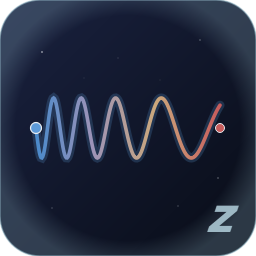
\includegraphics[width=4.2cm]{logo.png}}

\vspace{1.5cm}

{\Huge\textbf{Cosmological Distances}}\\[10pt]
{\LARGE From redshift to the age of the universe}\\[6pt]
{\large \textit{A course at three levels --- plain language, undergraduate, graduate}}

\vspace{2cm}

{\large\itshape With the interactive program \texttt{redshift\_distance\_gui.py}}

\vfill

{\large August 2026 edition}\\[4pt]
{\small (all numerical values re-checked with \emph{SageMath},
see appendix~\ref{chap:verif})}\\[6pt]
{\small \emph{Planck 2018} cosmology --- $\Hzero=67.66~\kms\,\Mpc^{-1}$
\quad $\Om=0.3111$ \quad $\OL=0.6889$}

\vspace{1.5cm}
\end{titlepage}

\vspace*{1cm}

\begin{tcolorbox}[colback=boxbgblue,colframe=accentcyan,arc=2mm]
\textbf{Purpose of this document.} This course presents, in detail and with
derivations, the physics that turns a \emph{cosmological redshift} $z$ into
several notions of distance and time, within the standard
$\Lambda\text{CDM}$ model constrained by the \emph{Planck 2018}
data~\cite{Planck2018}.

\medskip
Each notion is presented at three levels:

\medskip
\begin{tabular}{ll}
\textcolor{accentcyan}{\textbf{Level 1 --- Plain language}} &
analogies, mental images, no equations \\
\textcolor{accentsage}{\textbf{Level 2 --- Undergraduate}} &
calculus and integrals, no tensors \\
\textcolor{black}{\textbf{Level 3 --- Graduate}} &
general relativity, FLRW, complete derivations \\
\end{tabular}

\medskip
\textbf{Chapter 1} describes the graphical interface of
\texttt{redshift\_distance\_gui.py} in detail and explains every displayed
quantity, including the cryptic “TT,TE,EE+lowE+lensing+BAO” that names the
data combination behind the cosmological parameters used.

\medskip
All the numerical formulas are those implemented in the
\texttt{astropy.cosmology} library (\texttt{Planck18} cosmology)~\cite{astropy}.
\end{tcolorbox}

\tableofcontents
\clearpage

%==============================================================================
\chapter*{How to read this course}
\addcontentsline{toc}{chapter}{How to read this course}
%==============================================================================

This course is meant to be readable at several depths.

\begin{tcolorbox}[plain]
To grasp only \emph{the idea}, the blue boxes like this one are enough: no
equations, but the overall picture. Everything else can be skipped.
\end{tcolorbox}

\begin{tcolorbox}[undergrad]
With an undergraduate background in physics or engineering, the green boxes
add the essential formulas and short derivations using calculus and integrals
only --- no general relativity.
\end{tcolorbox}

\noindent\textbf{Level 3 (main text).} For a reader familiar with general
relativity (metric tensor, Einstein equations, index notation), the main text
gives the rigorous derivations, from the FLRW metric down to the cosmological
distances.

\begin{tcolorbox}[further]
Orange “Going further” boxes: historical background, current debates,
conceptual subtleties.
\end{tcolorbox}

\begin{tcolorbox}[numeric]
Green “Worked example” boxes: numbers for emblematic redshifts.
\end{tcolorbox}

\begin{tcolorbox}[gui]
Teal “In the program” boxes: what the quantity corresponds to in the
companion application \texttt{redshift\_distance\_gui.py}.
\end{tcolorbox}

\begin{tcolorbox}[warning]
Red “Warning” boxes: conceptual traps that popular accounts spread.
\end{tcolorbox}

\clearpage

%==============================================================================
\chapter*{Notation and conventions}
\addcontentsline{toc}{chapter}{Notation and conventions}
%==============================================================================

\begin{description}[leftmargin=2.4cm,labelwidth=2.2cm]
\item[Signature] The metric has signature $(-,+,+,+)$.
\item[Greek indices] $\mu,\nu \in \{0,1,2,3\}$, spacetime indices.
\item[Latin indices] $i,j \in \{1,2,3\}$, spatial indices.
\item[$c$] $\SI{299792.458}{\km\per\second}$ (exact by definition since 1983).
  We do not use the convention $c=1$.
\item[$\Hzero$] The Hubble constant today, in
  $\si{\km\per\second\per\mega\parsec}$. Planck 2018 value: $67.66$.
\item[$h$] Reduced Hubble parameter, $h \equiv \Hzero / (\SI{100}{\km\per\second\per\mega\parsec})$.
  Equal to $0.6766$ in Planck 2018.
\item[$z$] Cosmological redshift, dimensionless. Always positive for
  cosmological objects (the universe expands).
\item[$a(t)$] Scale factor, normalised so that $a(t_0) = 1$ today.
\item[$\Mpc$] The megaparsec, $1~\Mpc \approx \SI{3.086e19}{\km}
  \approx 3.262 \times 10^{6}~\ly$.
\item[$\ly$] The light-year, $1~\ly = \SI{9.461e12}{\km}$.
\item[$\Gly$] The giga-light-year, $1~\Gly = 10^{9}~\ly$.
\item[$\Gyr$] The gigayear ($10^{9}$ years).
\end{description}

\begin{remark}
Every distance introduced in this course is \emph{model dependent}: outside the
local universe ($z\ll 1$) there is no unique notion of distance. Turning a
redshift into a distance always presupposes a model --- here
$\Lambda\text{CDM}$ with the Planck 2018 parameters.
\end{remark}

\clearpage

%==============================================================================
\part{Reading the program and the Planck 2018 parameters}
%==============================================================================

%==============================================================================
\chapter[The graphical interface]{The graphical interface\\ \texttt{redshift\_distance\_gui.py}}
\label{chap:gui}
%==============================================================================

The program shipped with this course is a Qt6 application (PyQt6 + pyqtgraph)
that displays, for a redshift $z$ entered by the user, four cosmological
distances and several derived quantities, together with a log-log plot of these
distances against $z$. It is bilingual (French / English): the
\emph{Language} menu switches immediately.

\section{Overview}

The interface has four areas:

\begin{enumerate}[topsep=2pt]
\item \textbf{Header}: title and the cosmological reference line.
\item \textbf{Redshift panel}: the $z$ field and the preset buttons.
\item \textbf{Model panel}: spatial curvature $\Ok$ and the SH0ES comparison.
\item \textbf{Left panel}: four distances and the cosmological quantities;
\textbf{right panel}: an interactive plot of the four distances against $z$
(logarithmic axes), with a vertical cursor at the current $z$ and markers for
$z=1$, the maximum of $D_A$, GN-z11 and the CMB.
\end{enumerate}

\section{The subtitle line}
\label{sec:subtitle}

The line displayed under the title reads:

\begin{center}\itshape
Planck 2018 (TT,TE,EE+lowE+lensing+BAO) --- $\Hzero=67.66$~km/s/Mpc \quad
$\Om+\Omega_{\nu} = 0.31110$ \quad $\OL = 0.68885$ \quad
$\Omega_{\gamma} = 5.402\times10^{-5}$ \quad $t_{0} = 13.7869$~Gyr
\end{center}

\noindent It is not decorative: it states \emph{exactly} which model of the
universe the program uses. Let us decode it.

\begin{tcolorbox}[plain]
\textbf{In one sentence.} “The program uses the parameters of the universe
that the Planck space mission determined in 2018, by combining everything we
know about the relic radiation (the CMB) plus one independent external data
set.”
\end{tcolorbox}

\subsection{“Planck 2018”}

\emph{Planck} is the European Space Agency satellite launched in 2009, which
observed the cosmic microwave background (CMB) until 2013; its data were
released progressively. The final release, “Planck 2018 results” (published
in 2020 in \emph{A\&A}~641, A6), gives the most precise values to date of the
parameters of the standard cosmological model~\cite{Planck2018}.

\subsection{$\Hzero=67.66$~km/s/Mpc --- the Hubble constant}

This is the \emph{rate} at which the universe expands today. A galaxy at
$1~\Mpc$ from us (feeling no local force) recedes on average at
$67.66$~km/s. At $10~\Mpc$ it recedes ten times faster (Hubble's law).

\begin{tcolorbox}[warning]
$\Hzero$ has the dimension of an \emph{inverse time}: $\Hzero \approx
2.19\times 10^{-18}$~Hz. Its inverse, the \emph{Hubble time}, is
$1/\Hzero \approx 14.5$~Gyr, which is also the order of magnitude of the age of
the universe ($13.79$~Gyr) --- and that is no coincidence.
\end{tcolorbox}

\subsection{$\Om = 0.3111$ --- the total matter density}

This is the fraction of the total energy of the universe, today, in the form of
\emph{matter} (meaning “massive non-relativistic particles”), of all kinds:
\begin{itemize}[topsep=2pt]
\item $\Omega_b \approx 0.049$ ordinary \emph{baryons} (atoms, stars, gas,
  planets, and so on);
\item $\Omega_{\mathrm{cdm}} \approx 0.262$ \emph{cold dark matter}: massive
  collisionless particles of unknown nature.
\end{itemize}

So only $\sim 5\%$ of everything that weighs in the universe is made of known
matter; the remaining $\sim 26\%$ of matter is dark and detected only through
gravity.

\subsection{$\OL = 0.6889$ --- the cosmological constant (“dark energy”)}

The rest of the total energy ($\sim 69\%$) takes the form of “dark energy”,
attributed in the minimal model to a \emph{cosmological constant} $\Lambda$ (an
extra term in the Einstein equations). It produces the \textbf{acceleration} of
the expansion, observed for the first time in 1998~\cite{Riess1998,Perlmutter1999}.

\subsection{Why is $\Om + \OL \approx 1$?}

Because space is \textbf{flat}. The sum of all energy densities (matter +
radiation + $\Lambda$) must equal exactly 1 at zero curvature. Measurement
gives $\Om + \OL = 0.9999\pm 0.002$, which justifies assuming flatness. See
chapter~\ref{chap:lcdm}, section~\ref{sec:Ok}.

\subsection{“TT,TE,EE+lowE+lensing+BAO” --- the cryptic phrase}

This is the \textbf{list of data sets} combined by the Planck collaboration to
constrain all parameters simultaneously. Each acronym names an observation:

\begin{center}
\renewcommand{\arraystretch}{1.3}
\begin{tabular}{ll p{8.7cm}}
\toprule
\textbf{Acronym} & \textbf{Full name} & \textbf{What it measures} \\
\midrule
TT & Temperature--Temperature & Angular power spectrum of the CMB in
    \emph{intensity} (the temperature contrasts on the sky,
    $\Delta T/T \sim 10^{-5}$). The “historical” CMB measurement. \\
TE & Temperature--E-mode & Cross-correlation between temperature and E-mode
    polarisation (the curl-free component). \\
EE & E-mode--E-mode & The E-mode polarisation spectrum alone. Independent
    of TT. \\
lowE & low-$\ell$ E-mode polarisation & The EE spectrum at large angular
    scales ($\ell < 30$, i.e. angles $> 6^{\circ}$). Very sensitive to the
    reionisation optical depth. \\
lensing & CMB lensing & Gravitational lensing of the CMB by large-scale
    structure. The intervening structure slightly distorts the CMB map; that
    distortion is extracted statistically. \\
BAO & Baryon Acoustic Oscillations & Acoustic oscillations observed
    \emph{today} in the galaxy distribution (SDSS, BOSS, eBOSS). A peak at
    $\sim 150~\Mpc$ comoving, a relic of the sound waves of the primordial
    universe. \emph{External} to Planck, but combined with it. \\
\bottomrule
\end{tabular}
\end{center}

\begin{tcolorbox}[plain]
\textbf{Why combine everything?} A single observation constrains a few
parameters but leaves others free; combining independent measurements breaks
the degeneracies and yields a final precision much better than any single
measurement. Concretely, the CMB (TT, TE, EE) mostly fixes the global geometry
and the composition at recombination, while BAO calibrates the present-day
\emph{scale}. Together they constrain $\Hzero$, $\Om$ and $\OL$ to
$\sim 0.5\%$.
\end{tcolorbox}

\begin{tcolorbox}[undergrad]
\textbf{Angular power spectrum.} The CMB temperature map on the celestial
sphere is expanded in spherical harmonics:
\[
\frac{\Delta T}{T}(\theta,\phi) = \sum_{\ell,m} a_{\ell m}\,Y_{\ell m}(\theta,\phi),
\quad C_{\ell}^{TT} = \frac{1}{2\ell+1}\sum_m |a_{\ell m}|^{2}.
\]
$\ell$ is the \emph{multipole} (the spherical analogue of a Fourier mode);
$\ell\sim 200$ corresponds to an angle of $\sim 1^{\circ}$. The spectrum
$C_{\ell}^{TT}$ shows a series of acoustic peaks whose positions and amplitudes
depend on $\Om, \Omega_b, \OL, \Hzero, \ldots$; fitting the theoretical model to
the observed spectrum is what determines the parameters.
\end{tcolorbox}

\section{The displayed fields, one by one}

\subsection{The $z$ field and the presets}

\begin{tcolorbox}[gui]
The $z$ field accepts values between $0$ and $1500$, with five decimals; both
“.” and “,” work as decimal separator. The \textbf{preset} buttons load:
\begin{itemize}[topsep=2pt]
\item \textbf{M 87} ($z=0.00428$): the giant elliptical galaxy of the Virgo
  cluster, famous for hosting the first direct image of a supermassive black
  hole (EHT, 2019).
\item \textbf{3C 273} ($z=0.158$): the brightest quasar known, and one of the
  nearest.
\item \textbf{z = 1}: a teaching landmark, the typical limit of deep optical
  surveys.
\item \textbf{z = 2.34}: the running example used throughout this course.
\item \textbf{ULAS J1120} ($z = 7.085$): one of the most distant quasars known
  (Mortlock et al. 2011).
\item \textbf{GN-z11} ($z=10.6$): a galaxy observed by JWST in 2022, when the
  universe was only $\sim 435$~Myr old.
\item \textbf{Reionisation} ($z=20$): the epoch when the first stars reionise
  the neutral universe.
\item \textbf{CMB} ($z=1089.80$): the last-scattering surface.
\end{itemize}
\end{tcolorbox}

\subsection{Comoving distance}

\begin{tcolorbox}[gui]
\textbf{Quick definition.} The “present-day” distance between us and the
object, measured in the frame that expands with the universe. It is the
distance \emph{as it is today}, after expansion has carried the object away
from us.

\medskip
Rigorous definition and derivation: chapter~\ref{chap:Dc}.
\end{tcolorbox}

\subsection{Luminosity distance}

\begin{tcolorbox}[gui]
\textbf{Quick definition.} The distance one must put into the classical flux
formula $F = L/(4\pi D^2)$ to relate the observed flux $F$ to the intrinsic
luminosity $L$ of the source, despite the expansion. It is larger than the
“real” distance because expansion makes sources look fainter than they would
in a static universe.

\medskip
Rigorous definition and derivation: chapter~\ref{chap:DL}.
\end{tcolorbox}

\subsection{Angular diameter distance}

\begin{tcolorbox}[gui]
\textbf{Quick definition.} The distance one must put into $\theta = \ell/D$
(angular size = physical size / distance) to relate the observed angular size
to the physical size of the object.

\medskip
\textbf{The surprise.} At high $z$ ($z > 1.6$) this distance \emph{decreases}
with $z$! A more distant object can look \emph{larger} than a nearer one.

\medskip
Rigorous definition and derivation: chapter~\ref{chap:DA}.
\end{tcolorbox}

\subsection{Light-travel distance}

\begin{tcolorbox}[gui]
\textbf{Quick definition.} The \emph{intuitive} value: “the light took such and
such a time to arrive, so the object is at c $\times$ that time light-years”.
Bounded by $c\,t_0 \approx 13.79$~Gly (age $\times$ $c$).

\medskip
\textbf{But.} This distance has no proper metric meaning: it is neither the
present-day (comoving) distance nor the distance at emission (angular
diameter). It is merely the travel time times the speed of light. We give it
because it is so commonly quoted.

\medskip
Rigorous definition: chapter~\ref{chap:Dlt}.
\end{tcolorbox}

\subsection{Lookback time}

\begin{tcolorbox}[gui]
The \emph{lookback time} is the time (in years) elapsed since the light we
receive today left the source. For the CMB it is $\sim 13.79$~Gyr; for a galaxy
at $z=1$, $\sim 7.9$~Gyr.

\medskip
Relation to the light-travel distance: $D_{\text{lt}} = c \times t_L$.

\medskip
Rigorous definition: equation~\eqref{eq:tlookback}.
\end{tcolorbox}

\subsection{Age of the universe at $z$}

\begin{tcolorbox}[gui]
The age the universe had \emph{when the light was emitted}, counted from the
Big Bang ($t=0$). For the CMB it is $\sim 372\,000$ years; for $z=2.34$,
$\sim 2.8$~Gyr.

\medskip
The identity “lookback + age at $z$ = present age ($t_0 = 13.79$~Gyr)” is
therefore satisfied on every line.
\end{tcolorbox}

\subsection{Scale factor $a = 1/(1+z)$}

\begin{tcolorbox}[gui]
Recall: $a(t)$ is the dimensionless factor measuring the \emph{relative size}
of the universe at time $t$, normalised so that $a(t_0) = 1$ today.

\medskip
For light emitted at redshift $z$, $a_{\text{em}} = 1/(1+z)$.

\medskip
So at $z = 2.34$: $a_{\text{em}} = 0.2994$. The universe was about $3.34$ times
smaller (in every direction) when the light was emitted.
\end{tcolorbox}

\subsection{$E(z) = H(z)/\Hzero$}

\begin{tcolorbox}[gui]
The expansion rate at the epoch of emission, relative to today. This is the
function that gets integrated for \emph{all} the distances; the program
displays it so that one can see where the numbers come from. At $z=2.34$:
$E = 3.5056$, i.e. $H(z) = 237.2$~km/s/Mpc. At $z_{*}$: $E = 23\,053$.
Its exact form is given in~\eqref{eq:E_complete}.
\end{tcolorbox}

\subsection{The error bars}

\begin{tcolorbox}[gui]
Every distance and every duration is displayed as \emph{value $\pm$
uncertainty}, propagated from $\sigma(\Hzero) = 0.42$~km/s/Mpc and
$\sigma(\Om) = 0.0056$ by numerical partial derivatives, \textbf{taking the
correlation between the two into account} (section~\ref{sec:uncertainties}):
\[
\sigma_G^{2} = A^{2}\sigma_{\Hzero}^{2} + B^{2}\sigma_{\Om}^{2}
             + 2\rho\,A\,B\,\sigma_{\Hzero}\sigma_{\Om},
\qquad A = \pdv{G}{\Hzero},\quad B = \pdv{G}{\Om}.
\]
At $z = 2.34$: $D_{C} = 18.824 \pm 0.033$~Gly, i.e. $\pm0.17~\%$. The status bar
also shows what the same calculation would give \emph{without} the correlation
($\pm0.79~\%$): the factor of $4.5$ between the two is not a presentational
detail.
\end{tcolorbox}

\subsection{Curvature $\Ok$}

\begin{tcolorbox}[gui]
The \textbf{Curvature $\Ok$} field (range $\pm0.05$, default $0$) allows the
flat universe to be left behind. As soon as $\Ok \ne 0$ a fifth row appears: the
\textbf{transverse comoving distance} $D_{M}$, given by~\eqref{eq:DM} ---
$\sinh$ if $\Ok>0$, $\sin$ if $\Ok<0$. It is that one, not $D_{C}$, which then
enters $D_{L} = (1+z)D_{M}$ and $D_{A} = D_{M}/(1+z)$.

\medskip
The “flat ($\Ok = 0$)” button restores Planck 2018. Note that the present age
$t_{0}$ also changes with curvature ($13.744$~Gyr for $\Ok = +0.01$), and that
the status-bar check “$t_L + t_{\text{em}} = t_{0}$” refers to the age of the
\emph{current} model.
\end{tcolorbox}

\subsection{The SH0ES comparison}

\begin{tcolorbox}[gui]
The \textbf{“compare with SH0ES”} checkbox adds, under each value, the same
quantity computed with $\Hzero = 73.04$~km/s/Mpc (the local measurement, Riess
et al.~2022) together with the relative difference; the plot overlays the
corresponding dotted curves.

\medskip
Every distance shrinks by $7.4~\%$, and the durations with them. Compare that
with the $0.2~\%$ error bars: \textbf{the dominant uncertainty on a
cosmological distance today is not statistical, it is systematic.} That is
precisely what the Hubble tension is about.
\end{tcolorbox}

\subsection{Recession velocities --- all three}

\begin{tcolorbox}[gui]
The program displays \textbf{three} values, because they differ radically and
two of them are approximations:

\medskip
\begin{tabular}{lll}
\toprule
\textbf{Definition} & \textbf{at $z=2.34$} & \textbf{status} \\
\midrule
naive Doppler $v = cz$ & $701\,514$~km/s $=2.340\,c$ & valid if $z\ll1$ \\
relativistic Doppler & $250\,467$~km/s $=0.835\,c$ & inappropriate in cosmology \\
FLRW $v = \Hzero D_{C}$ & $390\,497$~km/s $=1.303\,c$ & \textbf{the right one} \\
\bottomrule
\end{tabular}

\medskip
The third one also exceeds $c$, and that is perfectly legitimate: it is not a
propagation speed \emph{through} space but the stretching rate of space itself.
See chapter~\ref{chap:vrec}.
\end{tcolorbox}

\subsection{The status-bar checks}

\begin{tcolorbox}[gui]
The status bar permanently displays two consistency checks:
$t_{L}(z) + t_{\text{em}}(z) = t_{0}$ (satisfied to within $10^{-4}$~$\mu$Gyr)
and the Etherington identity $D_{L}/[(1+z)^{2}D_{A}] = 1$ (satisfied to machine
precision). If either drifts, the backend has changed version or cosmology.
\end{tcolorbox}

\section{The log-log plot}

The horizontal axis is the redshift $z$ on a logarithmic scale; the vertical
axis is distance in Gly, also logarithmic. The four curves (comoving,
luminosity, angular diameter, light travel) are precomputed on
$z\in[10^{-3}, 1500]$ and cached on disk.

\textbf{Adaptive zoom}: the visible window follows the current $z$ as
$\bigl[z/30,\;8z\bigr]$, which keeps both nearby galaxies and the CMB legible.

The dotted vertical lines mark $z=1$, the maximum of $D_{A}$ (which follows
$\Ok$), GN-z11 ($z = 10.6$) and the CMB ($z = 1089.8$); the dash-dotted
horizontal lines mark $c\,t_{0}$ and the particle horizon.

%==============================================================================
\chapter{The preselected targets}
\label{chap:presets}
%==============================================================================

This chapter describes each of the eight clickable \emph{presets}, their
scientific interest and their place in the history of observational cosmology.

\section{M~87 --- the supermassive galaxy in Virgo ($z = 0.00428$)}

M~87 (NGC~4486) is a giant elliptical galaxy at the centre of the Virgo
cluster, about $55$~Mly away. Its redshift is very small because it belongs to
our immediate cosmic neighbourhood. It hosts a supermassive black hole
(M~87$^{\star}$) of about $6.5\times 10^{9}~M_{\odot}$, of which the
\emph{Event Horizon Telescope} published the first direct image in
2019~\cite{EHT2019}. It also emits a relativistic extragalactic jet observed
over several kpc.

Why as a preset? To anchor the user in the \emph{local} universe: at such a
small $z$ the four cosmological distances become nearly indistinguishable and
all equal $cz/\Hzero = 18.96~\Mpc = 61.8$~Mly (the exact values range from
$61.53$~Mly for $D_{A}$ to $62.06$~Mly for $D_{L}$).

\begin{tcolorbox}[warning]
\textbf{Do not confuse $\Mpc$ and Mly.} $cz/\Hzero = 18.96~\Mpc$, that is
$61.8$~Mly and not “$19$~Mly”.

\medskip
\textbf{And above all: that distance is wrong for M~87.} Direct measurements
(surface-brightness fluctuations, Cepheids) give $\sim 55$~Mly. The $\sim 12~\%$
difference is not a computational error: within the Virgo cluster the
\emph{peculiar velocity} of galaxies (several hundred km/s, caused by the
cluster's own gravity) adds to the Hubble flow and pollutes the redshift.
Converting $z$ into a distance only makes statistical sense beyond
$z \sim 0.03$, where the Hubble flow dominates peculiar motions. This is the
fundamental limitation of this program in the local universe.
\end{tcolorbox}

\section{3C~273 --- the first quasar ($z = 0.158$)}

3C~273 is the 273$^{\text{rd}}$ object of the \emph{Third Cambridge Catalogue of
Radio Sources}. In 1963 Maarten Schmidt, at the Mount Palomar telescope,
recognised its emission lines as hydrogen Balmer lines shifted by a factor
$1.158$. At visual magnitude $\sim 12.9$ it is the brightest quasar seen from
Earth~\cite{Schmidt1963}. Its bolometric luminosity reaches
$\sim 4\times 10^{46}$~erg/s, i.e. $\sim 10^{13}$ solar luminosities. At
$z=0.158$ the effects of expansion start to show: $D_{C} = 2.197$~Gly,
$D_{L} = 2.544$~Gly and $D_{A} = 1.897$~Gly --- three numbers already differing
by 34~\% between the extremes, while $z$ is still small.

\section{$z = 1$ --- a cosmological landmark}

At $z=1$ the universe was about $5.851$~Gyr old (a little less than half its
present age). This is the typical limit of deep optical galaxy surveys (before
JWST). The scale factor was $a = 0.5$, so the universe was \emph{twice
smaller} in every direction.

\section{$z = 2.34$ --- “cosmic noon”}

“Cosmic noon” denotes the epoch when star formation and quasar activity
peaked in the universe (typically $z \approx 1.5$ to $3$). The BOSS/eBOSS
spectroscopic surveys target that slice preferentially, and $z=2.34$ is a
reference point used in baryon acoustic oscillation (BAO) analyses through
quasars and the Lyman-$\alpha$ forest~\cite{Bautista2017}.

\section{ULAS J1120+0641 --- a quasar 749~Myr after the Big Bang ($z = 7.085$)}

Discovered in 2011 by the UKIDSS infrared survey, ULAS~J1120+0641 was for
several years the most distant known quasar~\cite{Mortlock2011}. Its central
black hole weighs $\sim 2\times 10^{9}~M_{\odot}$ although the universe was
only $749$~Myr old (the paper quotes $770$~Myr, obtained with the WMAP7
cosmology of the time; the $3~\%$ difference illustrates nicely that “the age
of an object” is a \emph{model-dependent} quantity). How such a massive black
hole formed so quickly remains one of the great theoretical challenges (direct
collapse? super-Eddington accretion? primordial seeds?).

\section{GN-z11 --- the galaxy at 435~Myr ($z = 10.6$)}

GN-z11 was first identified photometrically by Hubble in 2016 (Oesch~et~al.),
then confirmed spectroscopically by JWST in 2022/2023~\cite{Bunker2023}. At
$z = 10.603$ the universe was only $\sim 435$~Myr old and GN-z11 was already
forming stars at a high rate. It remains one of the most distant confirmed
objects (though JWST keeps finding more distant ones).

\section{Reionisation --- $z \approx 6$ to $20$}

This preset is not an object but an \emph{epoch}. After recombination (at
$z \approx 1100$) the hydrogen of the universe is neutral and opaque to stellar
UV photons. When the first stars ignite (Pop~III, $z \sim 30$), their UV
radiation progressively reionises the intergalactic hydrogen. The end of this
\emph{epoch of reionisation} (EoR) lies around $z \approx 5.5\text{-}6$. It is
detected indirectly through:
\begin{itemize}[topsep=2pt]
\item the CMB optical depth ($\tau \approx 0.054$, Planck~2018);
\item Lyman-$\alpha$ forest absorption in background quasars;
\item the 21~cm line of neutral hydrogen (HERA, and SKA in progress).
\end{itemize}

\section{CMB --- the last-scattering surface ($z_{*} = 1089.80$)}

The \emph{Cosmic Microwave Background} is the oldest radiation we can detect
directly. It comes from the epoch when the cooling universe became transparent
for the first time: free electrons and protons recombined into neutral
hydrogen, releasing the photons that have travelled ever since. See the
dedicated chapter~\ref{chap:cmb_observ}.

\clearpage

%==============================================================================
\part{Theoretical framework}
%==============================================================================

%==============================================================================
\chapter[Cosmological principle and FLRW]{The cosmological principle\\ and the FLRW metric}
\label{chap:flrw}
%==============================================================================

\section{The cosmological principle}

\begin{tcolorbox}[plain]
\textbf{The idea.} On very large scales (beyond a third of a billion
light-years), the universe looks the same everywhere and in every direction.
No centre, no edge, no privileged region. Clusters of galaxies look
statistically alike wherever one looks. This is an observation, not a
gratuitous assumption.
\end{tcolorbox}

\begin{tcolorbox}[undergrad]
\textbf{Restatement.} We postulate that there exists a frame (that of the
\emph{comoving observers}, attached on average to the clusters of galaxies) in
which two statistical properties hold on large scales:
\begin{itemize}[topsep=2pt]
\item \textbf{Homogeneity}: the mean density $\rho$ does not depend on position
  $\vec{x}$.
\item \textbf{Isotropy}: $\rho$, and any observable, does not depend on
  direction either.
\end{itemize}

If \emph{every observer} in the universe sees an isotropic universe, then by
Schur's theorem the universe is necessarily homogeneous, and the spatial metric
must have constant curvature.
\end{tcolorbox}

\begin{definition}[Cosmological principle]
There exists a preferred foliation of spacetime into spatial hypersurfaces
$\Sigma_t$ orthogonal to a reference congruence (the \emph{fundamental}, or
\emph{comoving}, observers), such that the induced metric on each $\Sigma_t$ is
\textbf{homogeneous} and \textbf{isotropic}.
\end{definition}

\section{The Friedmann--Lemaitre--Robertson--Walker metric}

\begin{tcolorbox}[plain]
\textbf{The rubber-sheet picture.} Consider a large rubber sheet with galaxies
drawn on it as dots. Stretching the sheet uniformly in every direction leaves
the dots fixed \emph{on the sheet} while they move apart from one another.
The “stretch factor” as a function of time is called $a(t)$. All of cosmic
expansion is contained in that simple idea.
\end{tcolorbox}

\begin{tcolorbox}[undergrad]
\textbf{Spatially flat FLRW metric.} In \emph{comoving} Cartesian coordinates
$(x,y,z)$ (which do not change in time for a fundamental observer), the spatial
line element at time~$t$ reads
\[
\dif s^{2}_{\text{spatial}} = a^{2}(t)\,\bigl(\dif x^{2} + \dif y^{2} + \dif z^{2}\bigr),
\]
i.e. Pythagoras with a factor $a(t)^{2}$ that dilates all distances with time.
Adding the time dimension:
\[
\dif s^{2} = -c^{2}\,\dif t^{2} + a^{2}(t)\,\bigl(\dif x^{2} + \dif y^{2} + \dif z^{2}\bigr).
\]
The minus sign on the time term reflects that we are doing relativity
(Lorentzian spacetime). In comoving spherical coordinates $(\chi, \theta, \phi)$:
\[
\dif s^{2} = -c^{2}\dif t^{2} + a^{2}(t)\,\bigl(\dif\chi^{2}
+ \chi^{2}\,(\dif\theta^{2} + \sin^{2}\theta\,\dif\phi^{2})\bigr).
\]
\end{tcolorbox}

A maximally symmetric (homogeneous and isotropic) Riemannian 3-manifold admits
exactly three spatial geometries: Euclidean space $\mathbb{E}^{3}$, the sphere
$S^{3}$, or hyperbolic space $\mathbb{H}^{3}$. Their common metric reads, in
generalised spherical coordinates $(\chi,\theta,\phi)$ centred on the observer:

\begin{equation}
\dif\sigma^{2} = \dif\chi^{2} + S_{k}^{2}(\chi)\,\dif\Omega^{2},
\quad \dif\Omega^{2} = \dif\theta^{2} + \sin^{2}\theta\,\dif\phi^{2},
\label{eq:dsigma}
\end{equation}

\noindent where $\chi$ is a dimensionless \emph{comoving radial coordinate} and
$S_{k}(\chi)$ encodes the spatial curvature of sign $k\in\{-1,0,+1\}$:

\begin{equation}
S_{k}(\chi) =
\begin{cases}
\sin\chi      & \text{if } k=+1 \text{ (sphere, closed universe)},\\
\chi          & \text{if } k=0 \text{ (flat space)},\\
\sinh\chi     & \text{if } k=-1 \text{ (open universe)}.
\end{cases}
\label{eq:Sk}
\end{equation}

\noindent Multiplying the hypersurfaces $\Sigma_t$ by a scale factor $a(t)$ and
using the cosmic time $t$ (the proper time of comoving observers) yields the
Friedmann--Lemaitre--Robertson--Walker (FLRW) metric:

\begin{equation}
\boxed{\;\dif s^{2} = -c^{2}\,\dif t^{2} + a^{2}(t)\,\bigl[\dif\chi^{2}
+ S_{k}^{2}(\chi)\,\dif\Omega^{2}\bigr].\;}
\label{eq:FLRW}
\end{equation}

\begin{remark}
The coordinate $\chi$ is \emph{comoving}: a galaxy that follows the Hubble flow
keeps a constant $\chi$. All the time dependence is in $a(t)$. This is the
formal statement of “the galaxies do not move, space expands”.
\end{remark}

\section{Comoving radial coordinate and instantaneous proper distance}

\begin{tcolorbox}[undergrad]
\textbf{Proper distance.} At fixed time $t$ ($\dif t = 0$), along a radial
direction ($\dif\Omega = 0$), the FLRW line element gives
$\dif s = a(t)\,\dif\chi$, hence
\begin{equation}
D_{p}(t) = a(t)\,\chi .
\label{eq:Dproper}
\end{equation}
This is the distance one would measure with a chain of rulers laid end to end
\emph{at one instant} of cosmic time. It is not directly observable --- no
signal travels instantaneously --- but it is the cleanest notion conceptually.
\end{tcolorbox}

Today, $a(t_0) = 1$, so the proper distance coincides with the comoving
distance: $D_{p}(t_0) = \chi$. That is exactly what the program calls the
\emph{comoving distance} $D_{C}$.

\section{Recession velocity and the Hubble flow}

Differentiating~\eqref{eq:Dproper} at fixed $\chi$:

\begin{equation}
v_{\text{rec}}(t) \eqdef \dot{D}_{p}(t) = \dot{a}(t)\,\chi
 = \frac{\dot{a}(t)}{a(t)}\,D_{p}(t) \eqdef H(t)\,D_{p}(t),
\label{eq:Hubble_law}
\end{equation}

\noindent which defines the \textbf{Hubble parameter}
$H(t) \equiv \dot a/a$, whose present value is $\Hzero$. Equation
\eqref{eq:Hubble_law} is Hubble's law, exact at all times and all distances
within FLRW --- with the important caveat that $v_{\text{rec}}$ is a rate of
change of a proper distance, not a velocity through space
(chapter~\ref{chap:vrec}).

%==============================================================================
\chapter{Cosmological redshift}
\label{chap:redshift}
%==============================================================================

\section{Observational definition}

\begin{tcolorbox}[plain]
\textbf{What is measured.} A galaxy emits light with the spectral lines of the
elements it contains --- hydrogen, calcium, oxygen. In the observed spectrum,
the H$\alpha$ line is no longer at $656.3$~nm: it is shifted towards the red,
say to $1969$~nm. The redshift is the relative shift:
$(1969-656.3)/656.3 = 2.0$. The more distant a galaxy, the larger its redshift.
\end{tcolorbox}

\begin{definition}[Redshift]
\begin{equation}
z \eqdef \frac{\lambda_{\text{obs}} - \lambda_{\text{em}}}{\lambda_{\text{em}}}
  = \frac{\lambda_{\text{obs}}}{\lambda_{\text{em}}} - 1 .
\label{eq:z_def}
\end{equation}
\end{definition}

For instance, if the H$\alpha$ line observed at $1969$~nm is emitted at
$656.3$~nm: $z = (1969 - 656.3)/656.3 = 2.00$. Redshifts are also measured
photometrically (from broad-band colours), less precisely.

\section{Derivation from the FLRW metric}

\begin{tcolorbox}[undergrad]
\textbf{Light travels on null geodesics.} Setting $\dif s^{2} = 0$ in
\eqref{eq:FLRW} for a radial ray:
\begin{equation}
c\,\dif t = -a(t)\,\dif\chi
\quad\Longrightarrow\quad
\chi = \int_{t_{\text{em}}}^{t_{0}} \frac{c\,\dif t}{a(t)} .
\label{eq:null_geodesic}
\end{equation}
Consider two successive wave crests, emitted at $t_{\text{em}}$ and
$t_{\text{em}} + \delta t_{\text{em}}$, received at $t_{0}$ and
$t_{0} + \delta t_{0}$. Both travel the same comoving distance $\chi$, hence
\[
\int_{t_{\text{em}}}^{t_{0}} \frac{c\,\dif t}{a}
= \int_{t_{\text{em}}+\delta t_{\text{em}}}^{t_{0}+\delta t_{0}} \frac{c\,\dif t}{a}
\quad\Longrightarrow\quad
\frac{\delta t_{0}}{a(t_0)} = \frac{\delta t_{\text{em}}}{a(t_{\text{em}})} .
\]
Since $\lambda = c\,\delta t$ and $a(t_0)=1$:
\end{tcolorbox}

\begin{equation}
\boxed{\;1 + z = \frac{a(t_{0})}{a(t_{\text{em}})} = \frac{1}{a_{\text{em}}} .\;}
\label{eq:z_FLRW}
\end{equation}

\noindent The redshift is therefore \emph{exactly} the factor by which the
universe has expanded since emission. It is not a velocity measurement: it is a
measurement of the expansion factor.

\begin{tcolorbox}[warning]
\textbf{“The galaxies fly away and their light is Doppler-shifted” is
misleading.} In FLRW the source is at rest in comoving coordinates. The
wavelength stretches \emph{because space stretches while the photon travels}.
Locally, the two descriptions agree (a Doppler shift is recovered for
$z\ll1$), but globally the expansion interpretation is the one that
generalises. See Bunn \& Hogg~\cite{Bunn2009} for a careful discussion.
\end{tcolorbox}

\section{Recession velocity and the apparent violation of $c$}
\label{sec:vrec_intro}

Writing $v = cz$ gives, for $z = 2.34$, $v = 2.34\,c$. This is not a violation
of relativity but a misuse of the Doppler formula: see
chapter~\ref{chap:vrec}, where the three definitions in circulation are
compared.

\section{Other redshifts}

A measured redshift is not purely cosmological. It combines:
\begin{itemize}[topsep=2pt]
\item the \textbf{cosmological} redshift $z_{\text{cosmo}}$ from expansion;
\item the \textbf{Doppler} redshift $z_{\text{D}}$ from the peculiar velocity of
  the source and of the observer (in a cluster, typically $\sim 300$~km/s, i.e.
  $z_{\mathrm{D}}\sim 10^{-3}$);
\item the \textbf{gravitational} redshift $z_{\text{grav}}$ from the potential
  well of the source (negligible except near compact objects).
\end{itemize}
They combine multiplicatively:
$(1+z_{\text{obs}}) = (1+z_{\text{cosmo}})(1+z_{\text{D}})(1+z_{\text{grav}})$.
This is exactly why M~87's redshift gives a distance $12~\%$ larger than direct
measurements.

\section{Thermal evolution}

Since wavelengths scale as $a$, a blackbody stays a blackbody with
$T \propto 1/a \propto (1+z)$. Hence the CMB temperature today,
$T_{0} = \SI{2.7255}{\kelvin}$, was $T = T_0 (1+z)$ in the past. At $z=1089$:
$T \approx 3000$~K, which is exactly the \emph{recombination} temperature ---
that is not a coincidence but the definition of $z_{*}$
(chapter~\ref{chap:cmb_observ}).

%==============================================================================
\chapter{The Friedmann equations}
\label{chap:friedmann}
%==============================================================================

\section{Stress-energy tensor of a perfect fluid}

The cosmological principle forces the matter content to be described, on
average, by a perfect fluid:

\begin{equation}
T^{\mu\nu} = \left(\rho + \frac{p}{c^{2}}\right)u^{\mu}u^{\nu} + p\,g^{\mu\nu},
\label{eq:Tmunu}
\end{equation}

\noindent with $\rho$ the energy density divided by $c^2$, $p$ the pressure and
$u^{\mu}$ the four-velocity of the comoving observers. Each component obeys an
equation of state $p = w\rho c^{2}$:

\begin{center}
\renewcommand{\arraystretch}{1.25}
\begin{tabular}{lcc}
\toprule
\textbf{Component} & $w$ & \textbf{Dilution} \\
\midrule
non-relativistic matter (baryons, CDM) & $0$ & $\rho \propto a^{-3}$ \\
radiation (photons, relativistic neutrinos) & $1/3$ & $\rho \propto a^{-4}$ \\
cosmological constant $\Lambda$ & $-1$ & $\rho = \text{const}$ \\
\bottomrule
\end{tabular}
\end{center}

\begin{tcolorbox}[plain]
\textbf{Why does radiation dilute faster than matter?} Because two effects
combine: the number of photons per unit volume falls as $a^{-3}$, like matter,
\emph{and} each photon loses energy as $a^{-1}$ through the redshift. Hence
$a^{-4}$ in total. That is why radiation dominated the early universe even
though it is negligible today.
\end{tcolorbox}

\section{Einstein equations with a cosmological constant}

\begin{equation}
G_{\mu\nu} + \Lambda g_{\mu\nu} = \frac{8\pi G}{c^{4}}\,T_{\mu\nu},
\qquad G_{\mu\nu} = R_{\mu\nu} - \tfrac{1}{2}R\,g_{\mu\nu}.
\label{eq:Einstein}
\end{equation}

Injecting the FLRW metric~\eqref{eq:FLRW} into~\eqref{eq:Einstein} gives two
independent equations, obtained from the $00$ and $ij$ components.

\section{First Friedmann equation}

\begin{equation}
\boxed{\;\left(\frac{\dot a}{a}\right)^{2} = H^{2}(t)
 = \frac{8\pi G}{3}\rho - \frac{k c^{2}}{a^{2}} + \frac{\Lambda c^{2}}{3}.\;}
\label{eq:Friedmann1}
\end{equation}

\begin{tcolorbox}[undergrad]
\textbf{Newtonian analogy.} For a test particle on the edge of a homogeneous
sphere of radius $R = a\chi$, energy conservation gives
$\tfrac12\dot R^{2} - GM/R = E$, i.e. exactly~\eqref{eq:Friedmann1} with
$-kc^2$ playing the role of the total energy. The analogy is not a derivation
(it ignores pressure and relativity) but it makes the equation memorable.
\end{tcolorbox}

\section{Second Friedmann equation (acceleration)}

\begin{equation}
\frac{\ddot a}{a} = -\frac{4\pi G}{3}\left(\rho + \frac{3p}{c^{2}}\right)
 + \frac{\Lambda c^{2}}{3}.
\label{eq:Friedmann2}
\end{equation}

\noindent Note that pressure \emph{slows} the expansion: in general relativity,
pressure gravitates. Only a component with $p < -\rho c^{2}/3$, i.e. $w<-1/3$,
can accelerate the expansion --- which is why dark energy needs $w \approx -1$.

\section{Continuity equation}

Combining the two Friedmann equations (or using $\nabla_\mu T^{\mu\nu}=0$):

\begin{equation}
\dot\rho + 3\frac{\dot a}{a}\left(\rho + \frac{p}{c^{2}}\right) = 0 .
\label{eq:continuity}
\end{equation}

\noindent With $p = w\rho c^{2}$ and constant $w$ this integrates to
$\rho \propto a^{-3(1+w)}$, which reproduces the dilution table above.

\section{Dimensionless form}

Dividing~\eqref{eq:Friedmann1} by $\Hzero^{2}$ and defining the density
parameters $\Omega_i \eqdef \rho_i/\rho_{c,0}$ with
$\rho_{c,0} = 3\Hzero^{2}/8\pi G$:

\begin{equation}
\boxed{\;\frac{H^{2}(z)}{\Hzero^{2}}
 = \Or\,(1+z)^{4} + \Om\,(1+z)^{3} + \Ok\,(1+z)^{2} + \OL \eqdef E^{2}(z).\;}
\label{eq:Ez}
\end{equation}

\noindent This single function $E(z)$ is what every distance integral in this
course uses. Its exact content in the program is detailed in
section~\ref{sec:E_real}.

%==============================================================================
\chapter{The \texorpdfstring{$\Lambda$}{Lambda}CDM model and the Planck 2018 parameters}
\label{chap:lcdm}
%==============================================================================

\section{Definition of the model}

\begin{tcolorbox}[plain]
\textbf{$\Lambda$CDM} is the “standard model” of cosmology. It says:
\begin{enumerate}[topsep=2pt]
\item hot Big Bang, expansion governed by general relativity;
\item \textbf{C}old \textbf{D}ark \textbf{M}atter: massive, slow,
  collisionless particles that only interact gravitationally;
\item dark energy represented by a cosmological constant $\Lambda$ that
  accelerates the expansion;
\item spatially flat universe.
\end{enumerate}
Six parameters suffice. It is the simplest model that fits \emph{all} the
observations.
\end{tcolorbox}

\section{Planck 2018 values}

\begin{center}
\renewcommand{\arraystretch}{1.25}
\begin{tabular}{lcl}
\toprule
\textbf{Parameter} & \textbf{Symbol} & \textbf{Value} \\
\midrule
Hubble constant today & $\Hzero$ & $67.66 \pm 0.42~\kms\,\Mpc^{-1}$ \\
Reduced Hubble parameter & $h$ & $0.6766$ \\
Total matter density & $\Om$ & $0.3111 \pm 0.0056$ \\
Baryon density & $\Omega_b h^{2}$ & $0.02242 \pm 0.00014$ \\
CDM density & $\Omega_c h^{2}$ & $0.11933 \pm 0.00091$ \\
Dark energy density & $\OL$ & $0.6889 \pm 0.0056$ \\
Curvature density & $\Ok$ & $\approx 0$ (within $\sim 2\sigma$) \\
Photon density & $\Omega_{\gamma}$ & $5.4020\times 10^{-5}$ (from $T_{0}$) \\
Equivalent radiation density & $\Or$ & $9.139\times 10^{-5}$
   \;{\footnotesize$=\Omega_{\gamma}(1+\tfrac{7}{8}(\tfrac{4}{11})^{4/3}N_{\text{eff}})$} \\
Neutrinos today & $\Omega_{\nu}$ & $1.4397\times 10^{-3}$
   \;{\footnotesize(non-relativistic)} \\
Effective species & $N_{\text{eff}}$ & $3.046$ \\
CMB temperature & $T_{0}$ & $2.7255 \pm 0.0006$ K \\
Age of the universe & $t_{0}$ & $13.787 \pm 0.020~\Gyr$ \\
CMB redshift & $z_{*}$ & $1089.80\pm 0.21$ \\
\bottomrule
\end{tabular}
\end{center}

\section{The $E(z)$ actually computed --- and why $\Om = 0.3111$ is not
astropy's $\Om$}
\label{sec:E_real}

This is the point most often glossed over, including by online calculators. The
program does \emph{not} use the two-term formula of popular accounts, but:

\begin{equation}
\boxed{\;E^{2}(z) = \Or(z)\,(1+z)^{4} + \Om^{\text{astropy}}(1+z)^{3}
       + \Ok(1+z)^{2} + \OL\;}
\label{eq:E_complete}
\end{equation}

\noindent with two subtleties:

\begin{enumerate}[topsep=3pt]
\item \textbf{The Planck paper's $\Om$ includes the neutrinos; astropy's does
not.} \texttt{Planck18} carries $\Om^{\text{astropy}} = 0.30966$ (baryons +
dark matter only) and $\Omega_{\nu} = 0.0014397$ separately. Their sum is
$0.31110$: exactly the “$\Om = 0.3111$” of Planck's Table~2. Neutrinos count
as \emph{matter} there because, with $\sum m_{\nu} = \SI{0.06}{\electronvolt}$,
they are non-relativistic today.

\item \textbf{$\Or$ depends on $z$}, because neutrinos change nature:
non-relativistic at $z=0$ (diluting as $(1+z)^{3}$), relativistic beyond
$z \sim 200$ (diluting as $(1+z)^{4}$). astropy writes
$\Or(z) = \Omega_{\gamma}\bigl[1 + \rho_{\nu}(z)/\rho_{\gamma}(z)\bigr]$ with
\[
\frac{\rho_{\nu}}{\rho_{\gamma}} = \frac{7}{8}\Bigl(\frac{4}{11}\Bigr)^{4/3}
\frac{N_{\text{eff}}}{3}\sum_{i} f\!\left(\frac{m_{i}c^{2}}{k_{B}T_{\nu}(z)}\right),
\quad
f(y) = \frac{120}{7\pi^{4}}\int_{0}^{\infty}\!\!
       \frac{x^{2}\sqrt{x^{2}+y^{2}}}{e^{x}+1}\,\dif x ,
\]
$f$ being evaluated through the analytic fit of Komatsu~et~al.~(2011).
\end{enumerate}

\begin{tcolorbox}[numeric]
\textbf{What does the simplified formula cost?} Comparing
$E_{\text{simple}} = \sqrt{\Om(1+z)^{3}+\OL}$ (with $\Om = 0.3111$) to the full
$E$:

\medskip
\begin{tabular}{rrrr}
\toprule
$z$ & full $E$ & simplified $E$ & difference \\
\midrule
$1$      & $1.78289$   & $1.78261$   & $-0.016~\%$ \\
$2.34$   & $3.50560$   & $3.50434$   & $-0.036~\%$ \\
$10.6$   & $22.0837$   & $22.0518$   & $-0.14~\%$ \\
$100$    & $573.82$    & $566.15$    & $-1.34~\%$ \\
$1089.8$ & $23\,053$   & $20\,094$   & $\mathbf{-12.8~\%}$ \\
\bottomrule
\end{tabular}

\medskip
Consequences for the observables: $D_{C}(z_{*})$ goes from $45.28$ to
$45.49$~Gly ($+0.46~\%$, harmless), but the \textbf{age of the universe at the
CMB goes from $372$~kyr to $479$~kyr}, i.e. $+29~\%$. In other words: for
distances the two-term formula is fine; for \emph{ages} at high $z$ it is
plainly wrong, because the age integral is dominated by the radiation era.
\end{tcolorbox}

\section{Observed curvature}
\label{sec:Ok}

Planck 2018 measures $\Ok = 0.0007 \pm 0.0019$ (consistent with zero at
$\sim 0.4\sigma$). Combining CMB+BAO gives $|\Ok| < 0.001$. All the
calculations in this course adopt $\Ok = 0$, but the program allows
$\Ok \neq 0$ to be explored (section~\ref{sec:DM}).

\section{Uncertainties and parameter correlation}
\label{sec:uncertainties}

\begin{tcolorbox}[plain]
\textbf{The idea.} The parameters of the model are not known exactly, so
neither are the distances. But one cannot simply add up the errors: the
parameters are \emph{tied together} by the measurement. An error on $\Hzero$
comes with a compensating error on $\Om$, and the distance moves far less than
one would think.
\end{tcolorbox}

\subsection{Two-parameter propagation}

\begin{tcolorbox}[undergrad]
For a quantity $G(\Hzero, \Om)$:
\begin{equation}
\sigma_G^{2} = A^{2}\sigma_{\Hzero}^{2} + B^{2}\sigma_{\Om}^{2}
             + 2\rho\,A\,B\,\sigma_{\Hzero}\sigma_{\Om},
\qquad A = \pdv{G}{\Hzero},\quad B = \pdv{G}{\Om},
\label{eq:propagation}
\end{equation}
where $\rho$ is the correlation coefficient between $\Hzero$ and $\Om$. The
third term vanishes \emph{only} if the two measurements are independent ---
which they are not.
\end{tcolorbox}

\subsection{Where $\rho = -0.976$ comes from}

One does not need Planck's full covariance matrix: it is enough to notice that
the combination
\[
\omega_{m} \equiv \Om h^{2} = 0.14239 \pm 0.00092
\]
is far better measured ($0.65~\%$) than $\Om$ ($1.8~\%$) or $h$ ($0.62~\%$)
separately. This is the signature of the \emph{geometric degeneracy}: the CMB
primarily constrains $\omega_m$ (which sets the acoustic scale), and separating
$\Om$ from $h$ comes only afterwards. Propagating~\eqref{eq:propagation} on
$\omega_m$:
\[
\left(\frac{\sigma_{\omega}}{\omega}\right)^{2}
 = \left(\frac{\sigma_{\Om}}{\Om}\right)^{2}
 + 4\left(\frac{\sigma_{h}}{h}\right)^{2}
 + 4\rho\,\frac{\sigma_{\Om}}{\Om}\frac{\sigma_{h}}{h}
\;\Longrightarrow\;
\boxed{\rho = -0.9763}
\]
(symbolic solution and numerical application in
\texttt{verif\_sage/verif\_courbure\_sigma.sage}).

\subsection{What difference it makes}

\input{table_sigma_en.tex}

\noindent Two lessons:

\begin{enumerate}[topsep=3pt]
\item \textbf{Ignoring $\rho$ overestimates the uncertainty by a factor of 2 to
5.} On $D_{C}$ at $z = 2.34$: $\pm0.17~\%$ instead of $\pm0.79~\%$.
\item \textbf{There is a “pivot” redshift.} The relative uncertainty on
$D_{C}$ decreases from $z=0$ ($\pm0.62~\%$, governed by $\Hzero$ alone, since
$D \simeq cz/\Hzero$) down to $z \approx 5$ ($\pm0.13~\%$), then rises again
slightly. Around that pivot the model predicts distances better than it knows
its own parameters.
\end{enumerate}

\begin{tcolorbox}[warning]
\textbf{These error bars do not contain everything.} They ignore
$\sigma(\Ok)$, $\sigma(T_{0})$, $\sigma(N_{\text{eff}})$ and
$\sigma(\sum m_{\nu})$ --- negligible here --- but above all they say nothing
about \textbf{model error}: if $\Lambda$CDM is wrong, no $\pm$ will reveal it.
And they are dwarfed by the Hubble tension (next section), which shifts
everything by $7~\%$.
\end{tcolorbox}

\section{The Hubble tension}

\begin{tcolorbox}[warning]
\textbf{A $\sim 5\sigma$ tension today.} Local measurements (the distance
ladder based on Cepheids and type Ia supernovae, the SH0ES
programme~\cite{Riess2022}) give
\[
\Hzero^{\text{loc}} = 73.04 \pm 1.04~\kms\,\Mpc^{-1},
\]
about $5\sigma$ above the Planck value $67.66$. This tension is one of the
major open questions of contemporary cosmology. No new physics is currently
accepted as the explanation.

\medskip
In the program, the “compare with SH0ES” checkbox shows the consequence:
every distance shrinks by $7.4~\%$, every age with it.
\end{tcolorbox}

\clearpage

%==============================================================================
\part{Cosmological distances}
%==============================================================================

%==============================================================================
\chapter{Comoving distance}
\label{chap:Dc}
%==============================================================================

\section{Hubble distance}

\begin{tcolorbox}[undergrad]
We define a “natural unit” of cosmological distance:
\[
D_{H} \eqdef \frac{c}{\Hzero}.
\]
Numerically, with $\Hzero = 67.66$~km/s/Mpc, $D_{H} = \num{4430.87}~\Mpc
= 1.3587$~Gpc $= 14.4516$~Gly. It is exactly the distance at which the FLRW
recession velocity $v = \Hzero D$ reaches $c$: the \emph{Hubble sphere}.
\end{tcolorbox}

\begin{equation}
D_{H} \eqdef \frac{c}{\Hzero} = \num{4430.87}~\Mpc = 1.3587~\text{Gpc}
     = 14.4516~\Gly .
\label{eq:DH}
\end{equation}

\begin{tcolorbox}[warning]
\textbf{Unit trap.} $1~\Mpc = 3.2616\times 10^{6}~\ly$, so $\num{4430.87}~\Mpc$
is \emph{not} $4.43$~Gly but $14.45$~Gly. Confusing the two divides every
distance by $3.26$; it is the most common mistake in hand calculations. The
ratio $D_{C}/z$ tends to $D_{H} = 14.45$~Gly as $z\to 0$, not to $4.4$.
\end{tcolorbox}

\section{Radial comoving distance}

\begin{tcolorbox}[plain]
\textbf{The idea.} We want the “present-day” distance separating us from the
distant object, as if we could freeze the universe now and stretch an
infinitely long ruler. That is the comoving distance.
\end{tcolorbox}

\begin{tcolorbox}[undergrad]
\textbf{Key formula.}
\[
D_{C}(z) = D_{H}\,\int_{0}^{z}\frac{\dif z'}{E(z')}
         \underset{\substack{\text{neglecting}\\\text{radiation}}}{\simeq}
           \frac{c}{\Hzero}\int_{0}^{z}\frac{\dif z'}{\sqrt{\Om(1+z')^{3} + \OL}}.
\]
The integral has no closed form but is trivial numerically (a few milliseconds
by Simpson's rule).

\medskip
\textbf{Careful}, the second expression is an \emph{approximation}: the full
$E(z)$ also contains radiation, see~\eqref{eq:E_complete} and
section~\ref{sec:E_real}. It is excellent up to $z\sim 10$ (error $< 0.04~\%$
on $D_{C}$) but off by $0.46~\%$ at $z_{*}$ --- and above all it would give an
age of the universe at the CMB of $479$~kyr instead of $372$~kyr.
\end{tcolorbox}

\begin{definition}
The \emph{radial comoving distance} $D_{C}$ of a source at redshift $z$ is the
\emph{present-day} ($t=t_0$) distance separating it from the observer, measured
along the line of sight at fixed cosmic time.
\end{definition}

From~\eqref{eq:null_geodesic} and~\eqref{eq:z_FLRW} (changing variable from $t$
to $z$ through $\dif t = -\dif a/(aH) = \dif z / [(1+z)H(z)]$):

\begin{equation}
\boxed{\;D_{C}(z) = D_{H}\int_{0}^{z}\frac{\dif z'}{E(z')}\;}
\label{eq:DC}
\end{equation}

\section{Transverse comoving distance}
\label{sec:DM}

\begin{equation}
D_{M}(z) =
\begin{cases}
\dfrac{D_{H}}{\sqrt{\Ok}}\,\sinh\!\left[\sqrt{\Ok}\,D_{C}(z)/D_{H}\right] & \Ok>0,\\[6pt]
D_{C}(z) & \Ok=0,\\[6pt]
\dfrac{D_{H}}{\sqrt{|\Ok|}}\,\sin\!\left[\sqrt{|\Ok|}\,D_{C}(z)/D_{H}\right] & \Ok<0.
\end{cases}
\label{eq:DM}
\end{equation}

\noindent In Planck 2018, $\Ok \approx 0$, hence $D_{M} = D_{C}$.

\begin{tcolorbox}[gui]
The program implements all three cases. As long as the “Curvature $\Ok$”
field is zero, $D_{M}$ is not displayed since it coincides with $D_{C}$; as
soon as one moves away from zero, it appears. Some values at $z = 2.34$
(verified in SageMath to five decimals):

\medskip
\begin{center}
\begin{tabular}{rrrr}
\toprule
$\Ok$ & $D_{C}$ (Gly) & $D_{M}$ (Gly) & $D_{M}/D_{C}$ \\
\midrule
$-0.01$ & $18.8928$ & $18.8390$ & $0.99715$ \\
$0$       & $18.8240$ & $18.8240$ & $1$ \\
$+0.01$ & $18.7560$ & $18.8087$ & $1.00281$ \\
\bottomrule
\end{tabular}
\end{center}

\medskip
Note the partial cancellation: at $\Ok = +0.01$, $D_{C}$ \emph{decreases} by
$0.36~\%$ (the dark-energy content changes) while the hyperbolic geometry
\emph{increases} $D_M$ by $0.28~\%$ relative to $D_C$. In total $D_{M}$ moves by
only $0.08~\%$: that is why curvature is so hard to measure from distances
alone.
\end{tcolorbox}

%==============================================================================
\chapter{Luminosity distance}
\label{chap:DL}
%==============================================================================

\section{Definition and motivation}

\begin{tcolorbox}[plain]
\textbf{The practical problem.} In astronomy we know the “true” luminosity of
certain objects (standard candles such as type Ia supernovae). We measure the
flux that reaches us. We would like to deduce the distance. The classical
formula $F = L/(4\pi D^{2})$ would work... in a static universe. In an
expanding one we need an \emph{effective} distance that keeps the formula
valid. That is the luminosity distance.
\end{tcolorbox}

\begin{tcolorbox}[undergrad]
\textbf{Three effects dilute the flux.}
\begin{enumerate}[topsep=2pt]
\item \emph{Geometric spreading.} The radiation spreads over a sphere of area
  $4\pi a_{0}^{2} D_{M}^{2}$.
\item \emph{Energy loss per photon.} $E_{\gamma} \to E_{\gamma}/(1+z)$.
\item \emph{Time dilation.} The photon arrival rate is divided by $(1+z)$.
\end{enumerate}
In total $F = L/[4\pi D_{M}^{2}\,(1+z)^{2}]$, hence $D_{L} = (1+z)\,D_{M}$.
\end{tcolorbox}

\begin{definition}
\begin{equation}
D_{L} \eqdef \sqrt{\frac{L}{4\pi F}}.
\label{eq:DL_def}
\end{equation}
\end{definition}

\section{Derivation from the FLRW metric}

\paragraph{(i) Geometric spreading.} At time $t_0$, the photons from a source
at comoving distance $D_{C}$ are spread over a sphere of proper area
$4\pi a_{0}^{2} D_{M}^{2}(z)$.

\paragraph{(ii) Energy shift.} Each photon loses a factor $(1+z)$ of energy.

\paragraph{(iii) Time dilation.} The arrival rate of photons is slowed by a
further factor $(1+z)$.

\noindent In total:

\begin{equation}
F = \frac{L}{4\pi D_{M}^{2}(z)\,(1+z)^{2}}.
\label{eq:F_obs}
\end{equation}

\begin{equation}
\boxed{\;D_{L}(z) = (1+z)\,D_{M}(z).\;}
\label{eq:DL}
\end{equation}

\section{Distance modulus and supernovae}

\begin{tcolorbox}[plain]
\textbf{How the acceleration of the expansion was discovered.} In 1998-1999 two
teams observed type Ia supernovae (which nearly all share the same absolute
luminosity) at $z\sim 0.5$. They looked \emph{fainter} than expected in a
decelerating universe, hence \emph{more distant}. The only explanation: the
expansion accelerates. Nobel Prize 2011 to Riess, Schmidt and Perlmutter.
\end{tcolorbox}

\begin{equation}
\mu(z) \eqdef m - M = 5\log_{10}(D_{L}/\text{Mpc}) + 25.
\label{eq:mu}
\end{equation}

%==============================================================================
\chapter{Angular diameter distance}
\label{chap:DA}
%==============================================================================

\section{Definition}

\begin{tcolorbox}[plain]
\textbf{The idea.} If I know the \emph{physical} size of an object (in km) and
I see its \emph{angular} size (in arcsec), the distance linking the two is the
angular diameter distance: $\theta = \ell/D_{A}$.
\end{tcolorbox}

\begin{tcolorbox}[undergrad]
\textbf{Key formula.} Since the light was emitted when the universe was smaller
by a factor $(1+z)$:
\[
D_{A}(z) = \frac{D_{M}(z)}{1+z} = \frac{D_{C}(z)}{1+z}~\text{(in a flat universe)}.
\]
\end{tcolorbox}

\begin{definition}
\begin{equation}
D_{A} \eqdef \frac{\ell}{\theta}.
\label{eq:DA_def}
\end{equation}
\end{definition}

\section{Derivation}

\begin{equation}
\boxed{\;D_{A}(z) = \frac{D_{M}(z)}{1+z}.\;}
\label{eq:DA}
\end{equation}

\section{The maximum of \texorpdfstring{$D_{A}$}{D\_A}}

\begin{tcolorbox}[warning]
\textbf{Counter-intuitive!} In $\Lambda$CDM, $D_{A}(z)$ rises to a maximum near
$z \approx 1.59$ and then \emph{decreases}. An object at $z = 5$ will generally
have a \emph{larger} angular size than an identical object at $z = 1$. The
reason: the object emitted its light at a time when it was physically
\emph{close} to us, so it subtends a large angle.
\end{tcolorbox}

\section{Etherington's reciprocity theorem}

\begin{theorem}[Etherington, 1933~\cite{Etherington1933}]
For any null geodesic in an arbitrary Lorentzian geometry:
\begin{equation}
\boxed{\;D_{L}(z) = (1+z)^{2}\,D_{A}(z).\;}
\label{eq:Etherington}
\end{equation}
\end{theorem}

%==============================================================================
\chapter{Lookback time and light-travel distance}
\label{chap:Dlt}
%==============================================================================

\section{Lookback time}

\begin{tcolorbox}[plain]
\textbf{The question.} How long has the light been travelling to reach us?
\end{tcolorbox}

\begin{tcolorbox}[undergrad]
\[
t_L(z) = \int_{0}^{z}\frac{\dif z'}{(1+z')H(z')}.
\]
Again an integral in $\dif z/E(z)$, this time weighted by $1/(1+z)$.
\end{tcolorbox}

\begin{equation}
t_{L}(z) = t_{0} - t_{\text{em}}(z) = \int_{0}^{z}\frac{\dif z'}{(1+z')\,H(z')}
        = \frac{1}{\Hzero}\int_{0}^{z}\frac{\dif z'}{(1+z')\,E(z')}.
\label{eq:tlookback}
\end{equation}

\section{Light-travel distance}

\begin{equation}
D_{\text{lt}}(z) \eqdef c\,t_{L}(z).
\label{eq:Dlt}
\end{equation}

\begin{tcolorbox}[warning]
$D_{\text{lt}}$ is the most \emph{intuitive} value but it has no proper metric
meaning. It is bounded by $c\,t_{0}\approx 13.79$~Gly whatever $z$: even for the
CMB ($z=1089.8$) it does not exceed that bound. The comoving distance, by
contrast, can exceed it (the CMB sits at $D_C \approx 45.3$~Gly).
\end{tcolorbox}

\section{Age of the universe at $z$}

\begin{equation}
t_{\text{em}}(z) = \int_{z}^{\infty}\frac{\dif z'}{(1+z')\,H(z')}.
\label{eq:t_z}
\end{equation}

%==============================================================================
\chapter{Summary}
%==============================================================================

\section{Summary table}

\begin{center}
\renewcommand{\arraystretch}{1.5}
\begin{tabular}{p{4.2cm}p{4.8cm}p{6cm}}
\toprule
\textbf{Distance} & \textbf{Formula} & \textbf{Use} \\
\midrule
Radial comoving $D_{C}$
 & $\displaystyle D_{H}\int_{0}^{z}\frac{\dif z'}{E(z')}$
 & the “present-day” distance of the source \\
Transverse comoving $D_{M}$
 & $D_{C}$ if $\Ok=0$
 & transverse scales, BAO \\
Luminosity $D_{L}$
 & $(1+z)\,D_{M}$
 & photometry, supernovae \\
Angular diameter $D_{A}$
 & $D_{M}/(1+z)$
 & apparent angular sizes \\
Light travel $D_{\text{lt}}$
 & $c\,t_{L}(z)$
 & popular accounts, $\le c\,t_{0}$ \\
\bottomrule
\end{tabular}
\end{center}

\section{Etherington identity}
\[
D_{L} = (1+z)^{2}\,D_{A}, \qquad D_{L} = (1+z)\,D_{M}, \qquad D_{A} = D_{M}/(1+z).
\]

\section{Asymptotic behaviour}

\paragraph{Small $z$ ($z\ll 1$).}
\[
D_{C} \simeq \frac{cz}{\Hzero}\Bigl[1 - \tfrac{1}{2}(1+q_{0})z + \mathcal{O}(z^{2})\Bigr],
\qquad
D_{L} \simeq \frac{cz}{\Hzero}\Bigl[1 + \tfrac{1}{2}(1-q_{0})z + \mathcal{O}(z^{2})\Bigr],
\]
with $q_{0} = \tfrac{1}{2}\Om - \OL = -\num{0.5334}$ (Planck 2018).

\paragraph{Large $z$.}
$D_{C}$ tends to the comoving distance to the particle horizon,
$\chi_{\text{hor}} = 46.20$~Gly in Planck 2018. Hence
$D_{A}\to \chi_{\text{hor}}/(1+z)$ (decreasing) and
$D_{L}\to \chi_{\text{hor}}(1+z)$ (growing linearly): it is
$\chi_{\text{hor}} = 46.2$~Gly that appears, not $D_{H} = 14.45$~Gly.
Check at $z_{*}$: $46.20/1090.8 = 0.0424$~Gly, against the exact value
$D_{A}(z_{*}) = 0.04152$~Gly (the $2~\%$ difference is because
$D_{C}(z_{*}) = 45.28$ has not quite saturated yet).

\clearpage

%==============================================================================
\part{Observed phenomena: CMB, observable universe, superluminal velocities}
%==============================================================================

%==============================================================================
\chapter{The cosmic microwave background}
\label{chap:cmb_observ}
%==============================================================================

\section{What is the CMB?}

\begin{tcolorbox}[plain]
\textbf{The oldest light.} The CMB (“Cosmic Microwave Background”) is the
oldest light one can see. It fills \emph{all} of space and arrives from every
direction at once, in the microwave range (millimetre wavelengths). It was
emitted when the universe was $\sim 372\,000$ years old (the Planck 2018 value;
the older WMAP figure of 380 000 years is still often quoted), and it has been
travelling for $\sim 13.8$ billion years.
\end{tcolorbox}

\begin{tcolorbox}[undergrad]
The CMB is an almost perfect blackbody at $T_{0} = 2.7255$~K, with relative
fluctuations $\Delta T/T \sim 10^{-5}$ that carry the cosmological information.
Its spectrum matches a blackbody to $\sim 10^{-9}$, making it the best measured
blackbody spectrum in all of physics.
\end{tcolorbox}

\section{Why we still see it today}

\begin{tcolorbox}[plain]
\textbf{The fog picture.} Consider a cloud of warm fog. As long as the cloud is
dense, light propagating in it is constantly absorbed and re-emitted: the cloud
is \emph{opaque}. When the cloud cools and thins out, at some point the
molecules no longer trap the light: the cloud becomes \emph{transparent}. All
the trapped light escapes at once, in every direction.

\medskip
That is what happened to the universe, at $z \approx 1100$. Before that, matter
was hot enough to ionise hydrogen into a plasma; photons were trapped by
scattering off free electrons (\emph{Thomson scattering}). At about
$T = 3000$~K hydrogen became neutral (\emph{recombination}): electrons stuck to
protons, and the photons could finally travel freely.

\medskip
This “release” of photons happens in every region of the universe at the same
epoch (to within the fluctuations). So \emph{from all around us}, at
$13.79$~billion light-years (in light-travel distance), we see this
“last-scattering surface”. Since the universe has been transparent ever
since, that radiation reaches us without further interaction.
\end{tcolorbox}

\begin{tcolorbox}[undergrad]
\textbf{Why $T \approx 3000$~K rather than $T \approx 13.6$~eV~$\approx 158\,000$~K
(the ionisation energy of hydrogen)?} Because photons vastly outnumber baryons
(the ratio is $n_{\gamma}/n_b \approx 1.6\times 10^{9}$). Even when the mean
energy $k_B T$ has fallen well below $13.6$~eV, the Wien tail of the Planck
distribution still holds enough UV photons to keep the gas ionised. The Saha
calculation puts recombination near $T \approx 3700$~K, refined by
non-equilibrium treatment (the Peebles equation) to
$T_{\text{rec}} \approx 3000$~K, i.e. $z_{*} = 1089.80$ according to
Planck~2018~\cite{Planck2018}.
\end{tcolorbox}

\section{Why exactly $z_{*} = 1089.80$?}

Blackbody radiation cools as $T \propto 1/a \propto (1+z)$. Knowing the present
CMB temperature $T_{0} = \SI{2.7255}{\kelvin}$ and the recombination
temperature of hydrogen ($T_{\text{rec}} \approx \SI{2970}{\kelvin}$ from the
Peebles equation):
\[
1 + z_{*} = \frac{T_{\text{rec}}}{T_{0}}
          = \frac{\num{2970}}{\num{2.7255}} \approx 1090.
\]
\textbf{So $z_{*}$ is not an arbitrary number}: it is the ratio between the
temperature at which the universe became transparent and the present-day
temperature of the radiation emitted then.

\section{Discovery of the CMB and successive missions}

\begin{description}[leftmargin=2.2cm]
\item[1948] Alpher, Herman and Gamow predict a relic radiation at $\sim 5$~K in
the hot Big Bang framework~\cite{Alpher1948}.
\item[1965] A.~Penzias and R.~Wilson accidentally detect an isotropic excess
noise at 4080~MHz at Bell Labs (the \emph{Holmdel Horn}). Nobel Prize
1978~\cite{Penzias1965}.
\item[1989-1993] The \emph{COBE} mission (NASA): confirms the perfect blackbody
spectrum (FIRAS) and detects the first anisotropies (DMR). Nobel Prize 2006
(Mather, Smoot)~\cite{Mather1994,Smoot1992}.
\item[2001-2010] The \emph{WMAP} mission (NASA): high-resolution mapping,
constrains $\Hzero$, $\Om$, $\OL$ to a few percent.
\item[2009-2013] The \emph{Planck} mission (ESA): the most precise to date, and
the source of the parameters used by this program~\cite{Planck2018}.
\end{description}

%==============================================================================
\chapter{Anatomy of the four curves}
\label{chap:curves}
%==============================================================================

The program plots the four distances against $z$ simultaneously. At small $z$
they are \emph{all superimposed}, then at large $z$ they diverge spectacularly.
This chapter explains why.

\section{The four equations together}

\begin{equation}
\label{eq:all_four}
\boxed{
\begin{aligned}
D_{C}(z)        &= \frac{c}{\Hzero}\,\int_{0}^{z}\frac{\dif z'}{E(z')} &&
\text{\small (comoving distance)} \\[4pt]
D_{L}(z)        &= (1+z)\,D_{M}(z) &&
\text{\small (luminosity distance)} \\[4pt]
D_{A}(z)        &= \frac{D_{M}(z)}{1+z} &&
\text{\small (angular diameter distance)} \\[4pt]
D_{\text{lt}}(z) &= c\,\int_{0}^{z}\frac{\dif z'}{(1+z')\,H(z')}
                  = \frac{c}{\Hzero}\,\int_{0}^{z}\frac{\dif z'}{(1+z')\,E(z')} &&
\text{\small (light travel)}
\end{aligned}
}
\end{equation}

\noindent where $E(z) = \sqrt{\Or(1+z)^{4} + \Om(1+z)^{3} + \Ok(1+z)^{2} + \OL}$.

\section{Why they coincide at small $z$}

\begin{tcolorbox}[plain]
\textbf{The intuition.} At very small $z$ the universe barely changed while the
photon travelled. So the precise definition of distance hardly matters: they
all tend to the same value, the one given by the usual Hubble law,
$D \approx cz/\Hzero$.
\end{tcolorbox}

\begin{tcolorbox}[undergrad]
\textbf{Leading order.} For $z \ll 1$, $E(z) \approx 1$ and
$(1+z)^{\pm 1} \approx 1$, so
\[
D_{C} \approx \frac{c}{\Hzero}\,z, \qquad
D_{L} \approx (1+z) D_{C} \approx D_{C}, \qquad
D_{A} \approx D_{C}/(1+z) \approx D_{C},
\]
and likewise $D_{\text{lt}} \approx (c/\Hzero)z \approx D_{C}$. \textbf{All four
coincide} at $cz/\Hzero$ to first order in $z$.
\end{tcolorbox}

\subsection{Second order (the first departures)}

\begin{align}
D_{C}(z)         &= \frac{c}{\Hzero}\Bigl[z - \tfrac{1}{2}(1+q_{0})\,z^{2} + \mathcal{O}(z^{3})\Bigr],
\label{eq:exp_DC}\\
D_{L}(z)         &= \frac{c}{\Hzero}\Bigl[z + \tfrac{1}{2}(1-q_{0})\,z^{2} + \mathcal{O}(z^{3})\Bigr],
\label{eq:exp_DL}\\
D_{A}(z)         &= \frac{c}{\Hzero}\Bigl[z - \tfrac{1}{2}(3+q_{0})\,z^{2} + \mathcal{O}(z^{3})\Bigr],
\label{eq:exp_DA}\\
D_{\text{lt}}(z) &= \frac{c}{\Hzero}\Bigl[z - \tfrac{1}{2}(2+q_{0})\,z^{2} + \mathcal{O}(z^{3})\Bigr],
\label{eq:exp_Dlt}
\end{align}

\noindent where $q_{0} = \tfrac{1}{2}\Om - \OL$ is the \emph{deceleration
parameter} (negative today, since the expansion accelerates):
\[
q_{0} = \tfrac{1}{2}(0.3111) - 0.6889 = -0.53335
\quad\text{(or $-0.5325$ including radiation, $q_0=\tfrac{\Om}{2}+\Or-\OL$).}
\]
Numerically, with $\Om = 0.3111$:
\[
\begin{aligned}
D_{C}/D_{H} &= z - 0.2333\,z^{2}, &\qquad D_{L}/D_{H} &= z + 0.7667\,z^{2},\\
D_{A}/D_{H} &= z - 1.2333\,z^{2}, &\qquad D_{\text{lt}}/D_{H} &= z - 0.7333\,z^{2}.
\end{aligned}
\]

\begin{tcolorbox}[warning]
\textbf{The classic trap.} Many texts give $z + \tfrac12(1-q_0)z^2$ for
$D_{C}$: that is the expansion of the \emph{luminosity} distance (the
Weinberg / Hubble--Sandage formula). The four coefficients above follow from
one another through the factors $(1+z)^{\pm1}$ and were re-derived by computer
algebra (appendix~\ref{chap:verif}); they differ by exactly one unit each,
which is visible in the numbers above.
\end{tcolorbox}

\section{Why they diverge at large $z$}

\begin{tcolorbox}[undergrad]
At large $z$ the dominant term of $E(z)$ is $E(z) \sim \sqrt{\Om}\,(1+z)^{3/2}$,
so
\[
\int_{0}^{z}\frac{\dif z'}{E(z')} \sim \frac{2}{\sqrt{\Om}}\Bigl[1 - (1+z)^{-1/2}\Bigr]
\xrightarrow[z\to\infty]{} \frac{2}{\sqrt{\Om}}.
\]
\textbf{$D_{C}$ therefore saturates} at a finite value: the comoving distance to
the particle horizon, $46.20$~Gly.

\medskip
\emph{Caution with that estimate}: it assumes matter domination \emph{over the
whole range}, which is false at small $z$ (where $\Lambda$ dominates) and at
very large $z$ (where radiation does). It gives $2D_{H}/\sqrt{\Om} = 51.8$~Gly
against the exact $46.20$~Gly: good to $12~\%$, enough to understand \emph{why}
the integral converges, not enough to quote a number.

\medskip
$D_{L} = (1+z) D_{M}$ \textbf{grows linearly with $z$}; $D_{A} = D_{M}/(1+z)$
\textbf{decreases towards zero}; $D_{\text{lt}} \le c\,t_{0} \approx 13.79$~Gly
\textbf{is bounded} (light can travel at most for the age of the universe).
\end{tcolorbox}

\subsection{Limiting values for the CMB ($z = 1089.8$)}

\begin{center}
\renewcommand{\arraystretch}{1.3}
\begin{tabular}{lr}
\toprule
\textbf{Distance} & \textbf{Value} \\
\midrule
$D_{C}(z_{*})$        & $45.285~\Gly$ \\
$D_{L}(z_{*})$        & $49\,397~\Gly$ \\
$D_{A}(z_{*})$        & $0.04152~\Gly = 41.5~\text{Mly}$ \\
$D_{\text{lt}}(z_{*})$ & $13.7865~\Gly$ \\
\bottomrule
\end{tabular}
\end{center}

\noindent These four numbers, all of which mean “the distance to the CMB”,
span \emph{six orders of magnitude} (from $\sim 40$~Mly to $\sim 50\,000$~Gly).
That is the divergence one sees on the plot.

\section{The maximum of $D_{A}$ near $z = 1.59$}

\begin{tcolorbox}[further]
The angular distance $D_A = D_{M}/(1+z)$ is the product of an increasing
function ($D_{M}$) and a decreasing one ($1/(1+z)$). Its derivative vanishes
where $\dif D_C / \dif z = D_C/(1+z)$, i.e. at $z = 1.592133$ in Planck 2018,
where $D_A = 5.84629$~Gly. Beyond that, increasing $z$ \emph{reduces} $D_A$.

\medskip
\textbf{Observable consequence.} A galaxy of physical size $30$~kpc at $z = 5$
appears angularly \emph{larger} than an identical galaxy at $z = 1$. This is
counter-intuitive and essential when interpreting JWST images.
\end{tcolorbox}

%==============================================================================
\chapter{Why redshift is not linear in distance}
\label{chap:nonlinear}
%==============================================================================

\section{The linear Hubble law and its range of validity}

\begin{tcolorbox}[plain]
\textbf{At small $z$.} For nearby galaxies ($z < 0.1$) we have the
\textbf{Hubble law}:
\[
v \approx \Hzero \times D, \qquad cz \approx \Hzero \times D.
\]
The recession velocity is proportional to distance, and so is the redshift. It
is a linear relation, observed by Hubble in 1929. In that regime, doubling the
distance doubles the redshift.

\medskip
\textbf{But it breaks down far away.} That neat linearity rests on two
assumptions that fail at large $z$:
\begin{enumerate}[topsep=2pt]
\item that the universe expands at the same rate during the whole light
  travel. False: $H(z)$ changes with time.
\item that the Doppler shift $v = cz$ applies. False: it is the expansion of
  space itself that shifts the wavelengths, not motion through space.
\end{enumerate}
\end{tcolorbox}

\section{The exact relation}

\begin{tcolorbox}[undergrad]
\textbf{The true relation between $z$ and comoving distance.}
\[
D_{C}(z) = \frac{c}{\Hzero}\int_{0}^{z}\frac{\dif z'}{E(z')},
\quad E(z) \simeq \sqrt{\Om(1+z)^{3} + \OL}
\quad\text{\small(without radiation, cf.~\eqref{eq:E_complete})}.
\]
At small $z$: $E(z) \approx 1$, so $D_C \approx (c/\Hzero)\,z$, linear.

\medskip
At large $z$ (matter-dominated regime): $E(z) \sim \sqrt{\Om}\,(1+z)^{3/2}$, so
the integral \emph{saturates}:
\[
\int_{0}^{z}\frac{\dif z'}{(1+z')^{3/2}}
  = 2\left[1 - (1+z)^{-1/2}\right] \xrightarrow[z\to\infty]{} 2.
\]
\textbf{Conclusion}: $D_C$ tends to a \emph{finite} value as $z\to\infty$,
called the \textbf{particle horizon radius}.
\end{tcolorbox}

\section{Numbers for a few redshifts}

\begin{center}
\renewcommand{\arraystretch}{1.3}
\begin{tabular}{rrrr}
\toprule
\textbf{$z$} & \textbf{$D_C$ (Gly)} & \textbf{$D_C / z$ (Gly)} & \textbf{$cz$ (km/s)} \\
\midrule
$0.01$   & $0.1442$          & $14.42$  & $2\,998$ \\
$0.1$    & $1.4108$          & $14.11$  & $29\,979$ \\
$0.5$    & $6.3484$          & $12.70$  & $149\,896$ \\
$1$      & $11.0751$         & $11.08$  & $299\,792$ \\
$2.34$   & $18.8240$         & $8.04$   & $701\,514$ \\
$5$      & $25.9173$         & $5.18$   & $1\,498\,962$ \\
$10.6$   & $31.8379$         & $3.00$   & $3\,177\,800$ \\
$1089.8$ & $45.2848$         & $0.0416$ & $326\,713\,821$ \\
$\infty$ & $46.2005$ (horizon) & $0$    & --- \\
\bottomrule
\end{tabular}
\end{center}

\noindent The ratio $D_C/z$ starts at $D_H = 14.45$~Gly at low $z$ and tends to
zero: the distance “saturates” while $z$ diverges. The $cz$ column is given
for reference only: beyond $z\sim 1$ it exceeds $c$ and is meaningless (see
chapter~\ref{chap:vrec}).

%==============================================================================
\chapter{The observable universe and its size}
\label{chap:observable}
%==============================================================================

\section{Definition}

\begin{tcolorbox}[plain]
\textbf{The observable universe} is the sphere centred on us containing every
region whose light has had time to reach us since the Big Bang. Beyond it, what
happens cannot (yet) influence us. So it is a ball, not the whole universe
(which may be infinite, or simply much larger).
\end{tcolorbox}

\section{Three radii not to be confused}

\begin{tcolorbox}[warning]
One often hears that “the observable universe has a radius of 13.8 billion
light-years”. \textbf{That is wrong.} Three very different numbers must be
distinguished.
\end{tcolorbox}

\begin{enumerate}
\item \textbf{The distance the light has travelled}: $c\,t_0 = 13.79$~Gly. It is
merely the age times the speed of light. \textbf{It is not the size of the
observable universe}: while the light travelled, space expanded.

\item \textbf{The comoving radius of the particle horizon}:
\[
D_{\text{hor}} = D_{H}\int_{0}^{\infty}\frac{\dif z'}{E(z')} = 46.2005~\Gly.
\]
This is the \emph{present-day} distance to the sphere from which the oldest
light comes (in practice the CMB, at $D_C \approx 45.3$~Gly, very close).
\textbf{This is the “size” of the observable universe in the modern sense.}

\item \textbf{The event horizon radius}: $16.58$~Gly comoving (computed in
appendix~\ref{chap:verif}). It is the limit beyond which a signal emitted
\emph{today} can never reach us, because of the accelerating expansion. See
\cite{Davis2004} for a clear discussion.
\end{enumerate}

\begin{tcolorbox}[undergrad]
\textbf{Why 46~Gly and not 13.8?} While the light travelled, space stretched by
a factor $(1+z)$ at each step. The CMB photon was emitted at
$D_A \approx 41.5$~Mly (the angular distance, i.e. the physical distance
\emph{at emission}) and travelled for $13.79$~Gyr, but during that time the
emitting matter was carried away by the expansion. Today that same matter sits
at $D_C = 45.3$~Gly:
\[
D_C = (1+z_*)\,D_A = 1090.8 \times 0.04152~\Gly \approx 45.28~\Gly.
\]
\end{tcolorbox}

\section{Total diameter}

The \emph{diameter} of the observable universe is therefore $\sim 92.4$~Gly, and
its \emph{volume} $\sim 4\times 10^{32}$ cubic light-years. It contains roughly
$2\times 10^{12}$ galaxies (JWST-era estimate).

\section{What lies beyond?}

\begin{tcolorbox}[further]
\textbf{We do not know, by definition.} But a few theoretical bounds:
\begin{itemize}[topsep=2pt]
\item if the universe is \emph{flat} (Planck 2018: $\Ok = 0$ to $\sim 0.5\%$),
  it may well be \emph{infinite};
\item if one insists on a finite universe, its total size must be at least
  $\sim 250$ times the observable part (from the constraint on $\Ok$);
\item beyond the event horizon, the accelerating expansion driven by $\Lambda$
  will keep new regions \emph{forever} out of reach.
\end{itemize}
\end{tcolorbox}

%==============================================================================
\chapter{Recession velocities and the superluminal universe}
\label{chap:vrec}
%==============================================================================

\section{The problem}

For $z = 2.34$ the program shows a “recession velocity” of
$\sim 700\,000$~km/s $= 2.34\,c$ under the naive Doppler definition. For the CMB
($z = 1089.8$) that value would be $\sim 1090\,c$. \textbf{What does that mean?
Does it violate relativity?}

\section{Three ways to compute a “recession velocity”}

\subsection{Classical Doppler: $v = cz$}

\begin{tcolorbox}[plain]
This is the everyday Doppler formula: a car receding at $30$~m/s shifts a
1000~Hz sound to $\sim 999.9$~Hz, i.e. $z\approx 10^{-7}$. From that one writes
$v = cz$ for light. \textbf{It is a very-low-$z$ approximation only.}
\end{tcolorbox}

For $z=2.34$: $v_{\text{Doppler}} = 2.34\,c$. That is what the first line of the
program shows --- as an approximation, not as the “true” velocity.

\subsection{Relativistic Doppler}

In special relativity the shift of a source receding radially at $v$ is
\[
1 + z = \sqrt{\frac{1 + v/c}{1 - v/c}}, \qquad
\frac{v}{c} = \frac{(1+z)^{2} - 1}{(1+z)^{2} + 1}.
\]
This formula is \emph{bounded by $c$} (as $z \to \infty$, $v\to c$). For
$z=2.34$: $v/c = (3.34^{2}-1)/(3.34^{2}+1) \approx 0.833$, i.e. $83\%$ of $c$.
For the CMB ($z\to 1090$): $v/c \to 0.999\,998\,3$.

\begin{tcolorbox}[warning]
\textbf{The relativistic Doppler formula is conceptually wrong in cosmology.}
It assumes the source moves \emph{through} a static Minkowski spacetime. But
the FLRW universe is not globally flat, and a comoving source does \emph{not}
move through space: space stretches between it and us. A different concept is
needed.
\end{tcolorbox}

\subsection{FLRW recession velocity: $v_{\text{rec}} = H(t)\,D_p(t)$}

\begin{tcolorbox}[undergrad]
\textbf{The “true” cosmological velocity.} For two comoving observers
separated by a proper distance $D_p(t) = a(t)\,\chi$ at time $t$,
\[
v_{\text{rec}}(t) = \dot D_p(t) = \dot a(t)\,\chi = H(t)\,D_p(t).
\]
This velocity is \emph{unbounded}: for large enough $D_p$, $v_{\text{rec}} > c$.
But it is not a propagation speed \emph{through} space: it is a
\emph{stretching} rate of space itself.
\end{tcolorbox}

Today, for the CMB:
\[
v_{\text{rec}}(t_0) = \Hzero \times D_C(\text{CMB})
   = 67.66~\text{km/s/Mpc} \times 13\,884~\Mpc
   = 939\,400~\text{km/s} = 3.134\,c.
\]
\textbf{So even the well-defined recession velocity is superluminal} for very
distant objects: not only the naive $cz \approx 1090\,c$, but also the
cosmologically correct $\sim 3\,c$.

\section{Why relativity is not violated}

\begin{tcolorbox}[plain]
\textbf{Einstein's rule, stated strictly.} No particle, no signal, no
information can propagate \emph{through space} faster than light. Measured by a
\emph{local} observer, the speed of an object in its immediate neighbourhood is
always $<c$.

\medskip
\textbf{But cosmic expansion is not motion through space.} It is space itself
that dilates. Two comoving observers are \emph{at rest}: their comoving
coordinate $\chi$ does not change. Only the physical distance between them
grows with time. Nothing travels at $1.3\times 10^{6}$~km/s past anybody.
\end{tcolorbox}

\begin{tcolorbox}[undergrad]
\textbf{Rigorous statement.} In general relativity the limit $c$ applies
\emph{locally}, within the light cone at each point. Relativity does not forbid
two regions of space from separating at an arbitrarily large coordinate
velocity. The rule $v\le c$ is a statement of \emph{special} relativity, i.e.
of a globally Minkowski spacetime. In cosmology spacetime is curved; velocities
between distant points have no unique definition, and the one we use ($H D$) may
exceed~$c$.
\end{tcolorbox}

\section{Are superluminal galaxies observable?}

\textbf{Yes.} Surprisingly, we do see objects whose recession velocity exceeds
$c$ today. The condition for a signal emitted today by an object at $D_p$ to
reach us eventually is not $v_{\text{rec}} \le c$ but that $D_p$ be
\emph{smaller than the event horizon}. Numerically,
$D_{\text{event}} = 16.58$~Gly, whereas the sphere where
$v_{\text{rec}}(t_0) = c$ (the Hubble sphere) is at $D_H \approx 14.45$~Gly. So
galaxies in the shell between $14.45$ and $16.58$~Gly recede faster than light
yet emit light that will eventually reach us (heavily redshifted). See
\cite{Davis2004} for details.

\clearpage

%==============================================================================
\part{Worked examples}
%==============================================================================

%==============================================================================
\chapter{Numbers for a few emblematic redshifts}
%==============================================================================

\section{The running example \texorpdfstring{$z=2.34$}{z=2.34}}

\begin{tcolorbox}[numeric]
\textbf{Input.} $z=2.34$, Planck 2018 cosmology.

\medskip
\noindent\textbf{Results.}
\begin{itemize}[topsep=2pt]
  \item $D_{C} = D_{M} = \num{18.824} \pm \num{0.033}~\Gly$
  \item $D_{L} = (1+z)\,D_{M} = \num{62.87} \pm \num{0.11}~\Gly$
  \item $D_{A} = D_{M}/(1+z) = \num{5.6359} \pm \num{0.0098}~\Gly$
  \item $t_{L} = \num{10.988}~\Gyr$,\quad $D_{\text{lt}} = c\,t_{L} = \num{10.988}~\Gly$
  \item $t_{\text{em}} = t_{0} - t_{L} = \num{2.7991}~\Gyr$
  \item $a(t_{\text{em}}) = 1/(1+z) = \num{0.2994}$
  \item $E(z) = 3.5056$, i.e. $H(z) = 237.2$~km/s/Mpc
  \item recession velocity (FLRW) $v = 1.303\,c$
\end{itemize}

\medskip
\noindent\textbf{Interpretation.} The light was emitted when the universe was
$2.80~\Gyr$ old (out of $13.79$). At that moment the object was at
$D_{A}=5.64$~Gly. The light travelled for $10.99$~Gyr; meanwhile the universe
expanded by a factor $3.34$ and the object now lies at $D_{C}=18.82$~Gly.
$D_{L}$ reaches $62.87$~Gly because of the three cumulative effects.
\end{tcolorbox}

\section{The case \texorpdfstring{$z=1$}{z=1}}

\begin{tcolorbox}[numeric]
$D_{C} = \num{11.075}~\Gly$,\quad $D_{L} = \num{22.150}~\Gly$,\quad
$D_{A} = \num{5.538}~\Gly$,\quad
$t_{L} = \num{7.9355}~\Gyr$,\quad $t_{\text{em}} = \num{5.8513}~\Gyr$.
\end{tcolorbox}

\section{The case \texorpdfstring{$z=10.6$}{z=10.6} (GN-z11)}

\begin{tcolorbox}[numeric]
$D_{C} = \num{31.838}~\Gly$,\quad $D_{L} = \num{369.32}~\Gly$,\quad
$D_{A} = \num{2.7446}~\Gly$,\quad
$t_{L} = \num{13.3517}~\Gyr$,\quad $t_{\text{em}} = \num{435}~\text{Myr}$.

\medskip
GN-z11 is one of the most distant spectroscopically confirmed galaxies (JWST
2022/23); in Planck 2018 cosmology the universe was $435$~Myr old. The often
quoted “$\sim 400$~Myr” comes from earlier cosmologies and from $z = 11.09$
(the 2016 photometric estimate, corrected to $z = 10.60$ by JWST spectroscopy).
\end{tcolorbox}

\section{The case \texorpdfstring{$z=1089.8$}{z=1089.8} (CMB)}

\begin{tcolorbox}[numeric]
$D_{C} = \num{45.285}~\Gly$,\quad $D_{L} = \num{49397}~\Gly$ (enormous),\quad
$D_{A} = \num{0.04152}~\Gly = \num{41.5}~\text{Mly}$,\quad
$t_{L} = \num{13.7865}~\Gyr$,\quad $t_{\text{em}} = \num{372}~\text{kyr}$.

\medskip
The comoving distance to the CMB is very close to the particle horizon radius.
The angular distance is only $\sim 42$~Mly: one causal patch of the CMB
subtends $\sim 1^{\circ}$ on the sky (the first acoustic peak).
\end{tcolorbox}

\clearpage

%==============================================================================
\chapter{Numerical implementation}
%==============================================================================

\section{Evaluating the integrals}

The integral~\eqref{eq:DC} \textbf{has no} expression in elementary functions in
$\Lambda$CDM: the substitution $u = (1+z)^{-3/2}$ leaves an irreducible factor
$u^{-2/3}$, and the closed form involves a hypergeometric function (or an
incomplete elliptic integral). So it is computed numerically.

\paragraph{What does have a closed form: the age.} In flat $\Lambda$CDM
neglecting radiation ($\Or = 0$), the \emph{age} integral can be done exactly,
because the extra weight $1/(1+z)$ makes the substitution complete:

\begin{equation}
\boxed{\;t(z) = \frac{2}{3\,\Hzero\sqrt{\OL}}\;
\arcsinh\!\left[\sqrt{\frac{\OL}{\Om}}\;(1+z)^{-3/2}\right]\;}
\label{eq:age_closed}
\end{equation}

\noindent Numerical check ($\Om = 0.3111$, $\OL = 0.6889$,
$1/\Hzero = 14.4516$~Gyr):
\[
t(0) = 13.7915~\Gyr, \quad t(1) = 5.8555~\Gyr, \quad
t(2.34) = 2.8025~\Gyr,
\]
against the exact values (\emph{with} radiation) $13.7869$, $5.8513$ and
$2.7991$~Gyr. The agreement is better than $0.04~\%$ as long as
$z \lesssim 10$; at $z_{*}$ the formula gives $479$~kyr instead of $372$~kyr,
because it ignores the radiation era. This closed form was verified
symbolically and then numerically (appendix~\ref{chap:verif}); it is handy for
checking a result of the program by hand.

\begin{tcolorbox}[warning]
The prefactor is $\tfrac{2}{3\sqrt{\OL}}$, not $\tfrac{2}{\sqrt{\OL}}$; and
this expression gives the \emph{age} $t(z)$, not the comoving distance. The
lookback time follows as $t_{L}(z) = t(0) - t(z)$.
\end{tcolorbox}

\section{Python listing}

\begin{verbatim}
from astropy.cosmology import Planck18 as cosmo
from astropy import units as u, constants as const

z = 2.34
D_C  = cosmo.comoving_distance(z).to(u.Glyr)
D_M  = cosmo.comoving_transverse_distance(z).to(u.Glyr)
D_L  = cosmo.luminosity_distance(z).to(u.Glyr)
D_A  = cosmo.angular_diameter_distance(z).to(u.Glyr)
t_L  = cosmo.lookback_time(z).to(u.Gyr)
D_lt = (t_L * const.c).to(u.Glyr)
age  = cosmo.age(z).to(u.Gyr)

# the three "recession velocities" (see the dedicated chapter)
c_kms  = const.c.to_value(u.km / u.s)
v_cz   = c_kms * z                                   # naive Doppler
v_sr   = c_kms * ((1+z)**2 - 1) / ((1+z)**2 + 1)     # relativistic Doppler
v_flrw = cosmo.H0.value * cosmo.comoving_distance(z).to_value(u.Mpc)   # FLRW
\end{verbatim}

\begin{tcolorbox}[warning]
The giga-light-year unit is spelled \texttt{u.Glyr} in \texttt{astropy} (from
\texttt{lyr}), \emph{not} \texttt{u.Gly}: the latter does not exist and raises
an \texttt{AttributeError}. Likewise \texttt{u.lyr}, not \texttt{u.ly}.
\end{tcolorbox}

\noindent The complete program, with a Qt6 interface reproducing the log-log
plot and all four distances as functions of $z$, is
\texttt{redshift\_distance\_gui.py}.

\clearpage

%==============================================================================
\part{Appendices}
%==============================================================================

\appendix

%==============================================================================
\chapter{Physical constants}
%==============================================================================

\begin{center}
\renewcommand{\arraystretch}{1.3}
\begin{tabular}{lll}
\toprule
\textbf{Constant} & \textbf{Symbol} & \textbf{Value} \\
\midrule
Speed of light & $c$ & $\SI{299792.458}{\km\per\second}$ (exact) \\
Newton's constant & $G$ & $\SI{6.67430e-11}{\meter\cubed\per\kg\per\second\squared}$ \\
Parsec & $\text{pc}$ & $\SI{3.0857e13}{\km}$ \\
Julian year & $\text{yr}$ & $\SI{3.15576e7}{\second}$ \\
Light-year & $\ly$ & $\SI{9.4607e12}{\km}$ \\
Megaparsec & $\Mpc$ & $\SI{3.0857e19}{\km} = \num{3.2616e6}~\ly$ \\
\bottomrule
\end{tabular}
\end{center}

%==============================================================================
\chapter{Independent verification of the calculations (SageMath)}
\label{chap:verif}
%==============================================================================

This course and the program rely on \texttt{astropy.cosmology.Planck18}.
Trusting a single computation chain is bad practice, so every value has been
\textbf{recomputed from scratch in SageMath}, without astropy, at extended
precision.

\section{Method}

\begin{enumerate}[topsep=3pt]
\item \textbf{Rebuilding the parameters} from the CODATA 2022 constants and
$(\Hzero, \Om, T_{0}, N_{\text{eff}}, m_{\nu})$ alone:
\[
\rho_{c,0} = \frac{3\Hzero^{2}}{8\pi G},\quad
\Omega_{\gamma} = \frac{a_{B}T_{0}^{4}}{\rho_{c,0}c^{2}},\quad
a_{B} = \frac{\pi^{2}k_{B}^{4}}{15\hbar^{3}c^{3}},\quad
T_{\nu 0} = \Bigl(\tfrac{4}{11}\Bigr)^{1/3}T_{0}.
\]
\item \textbf{Neutrinos through the exact Fermi--Dirac integral}
$f(y) = \frac{120}{7\pi^{4}}\int_{0}^{\infty}\frac{x^{2}\sqrt{x^{2}+y^{2}}}{e^{x}+1}\dif x$,
instead of the Komatsu~et~al.~(2011) analytic fit used by astropy.
\item \textbf{Integrals} $D_{C}$, $t_{L}$, $t(z)$ by adaptive \texttt{mpmath}
quadrature at 25 significant digits, with the substitution $u = 1/(1+z)$ for
the infinite bound of the age.
\item \textbf{Series expansions} and the closed form of the age verified by
\emph{computer algebra} (symbolic Sage), not only numerically.
\end{enumerate}

\section{Rebuilt parameters}

\begin{center}
\renewcommand{\arraystretch}{1.25}
\begin{tabular}{lll}
\toprule
\textbf{Quantity} & \textbf{SageMath (rebuilt)} & \textbf{astropy} \\
\midrule
$\rho_{c,0}$ & $8.598814\times10^{-30}$ g/cm$^{3}$ & $8.598814\times10^{-30}$ \\
$\Omega_{\gamma}$ & $5.4020151\times10^{-5}$ & $5.4020151\times10^{-5}$ \\
$T_{\nu 0}$ & $1.9453688$~K & $1.9453688$~K \\
$\Omega_{\nu}$ (exact Fermi--Dirac) & $1.4397093\times10^{-3}$ &
   $1.4396743\times10^{-3}$ (Komatsu) \\
$\OL$ (from flatness) & $0.68884627$ & $0.68884631$ \\
$\Om + \Omega_{\nu}$ & $0.31109971$ & $0.31109968$ \\
$t_{0}$ & $13.786892$~Gyr & $13.786885$~Gyr \\
$D_{H} = c/\Hzero$ & $14.4515552$~Gly & $14.4515552$~Gly \\
\bottomrule
\end{tabular}
\end{center}

\noindent The Komatsu fit departs from the exact integral by $-0.0024~\%$ at
$z=0$ and at most $0.12~\%$ (around $z\sim 10$, in the
relativistic/non-relativistic transition of the neutrinos). Since
$\Omega_{\nu} \sim 10^{-3}$, the effect on the observables stays below
$1.5\times10^{-5}$.

\section{Agreement between the two computation chains}

\input{table_reference_en.tex}

\noindent \textbf{Conclusion:} the two calculations, independent from the
choice of constants down to the quadrature method, agree far better than the
uncertainty of the cosmological parameters themselves ($\sim 0.5~\%$, and
$\sim 7~\%$ if one accounts for the Hubble tension). \textbf{The program is
numerically reliable}; its limitation is the \emph{model}, not the arithmetic.

\section{Independent checks}

\begin{itemize}[topsep=3pt]
\item \textbf{Etherington} $D_{L} = (1+z)^{2}D_{A}$: verified to
$2\times10^{-16}$ (machine precision) over the whole range.
\item \textbf{Time conservation} $t_{L}(z) + t_{\text{em}}(z) = t_{0}$: verified
to $2\times10^{-10}$~Gyr.
\item \textbf{Closed form of the age}~\eqref{eq:age_closed}: recovered to
$10^{-9}$ by comparison with the quadrature, for the model without radiation.
\item \textbf{Series expansions}~\eqref{eq:exp_DC}--\eqref{eq:exp_Dlt}: the four
coefficients $-\tfrac{1+q_{0}}{2}$, $+\tfrac{1-q_{0}}{2}$,
$-\tfrac{3+q_{0}}{2}$, $-\tfrac{2+q_{0}}{2}$ are obtained by symbolic
\texttt{series()} and confirmed numerically at $z=0.1$ ($D_{C}$: $1.41076$
against the exact $1.41077$).
\item \textbf{Maximum of $D_{A}$}: root of $(1+z)/E(z) = D_{C}(z)/D_{H}$, giving
$z = 1.592133$ and $D_{A} = 5.84629$~Gly, identical by both methods to
$4\times10^{-7}$.
\item \textbf{Horizons}: particle horizon $46.2005$~Gly, Hubble sphere
$14.4516$~Gly, event horizon $16.5808$~Gly
$= D_{H}\int_{1}^{\infty} \dif a/[a^{2}E(a)]$.
\item \textbf{Correlation} $\rho(\Hzero,\Om) = -0.9763$, derived symbolically
from the constraint on $\omega_m$ (section~\ref{sec:uncertainties}).
\item \textbf{Curvature}: for $\Ok = -0.01$, $0$, $+0.01$ at $z = 0.5$, $2.34$,
$10.6$ and $1089.8$, the values of $D_{C}$, $D_{M}$, $D_{L}$ and $D_{A}$ agree
to \textbf{five decimals} between the program and SageMath.
\end{itemize}

\section{The scripts}

They ship with the program, in \texttt{verif\_sage/}:

\begin{description}[leftmargin=3.6cm,labelwidth=3.4cm]
\item[\texttt{verif\_cosmo.sage}] full reconstruction and reference table
(runtime $\sim 50$~s);
\item[\texttt{verif\_DL\_symbolique.sage}] computer-algebra check of the series
expansions and of the closed form of the age;
\item[\texttt{verif\_courbure\_sigma.sage}] symbolic derivation of the
correlation $\rho(\Hzero,\Om)$ and check of the distances with curvature.
\end{description}

\noindent Running them:
\begin{verbatim}
sage verif_sage/verif_cosmo.sage
\end{verbatim}

%==============================================================================
\chapter{Annotated bibliography and sources}
\label{chap:biblio}
%==============================================================================

All the numerical values in this course come from the Planck 2018 cosmology as
implemented in \texttt{astropy.cosmology.Planck18}.

\section{Measurement of the cosmological parameters}

\paragraph{Planck 2018 (reference parameters).}
N.~Aghanim \emph{et al.} (Planck Collaboration), \emph{Planck 2018 results.
VI. Cosmological parameters}, Astron.\ Astrophys.\ \textbf{641}, A6 (2020).
\href{https://doi.org/10.1051/0004-6361/201833910}{DOI}~|
\href{https://arxiv.org/abs/1807.06209}{arXiv:1807.06209}.
The primary source of the parameters used (Table 2, column
TT,TE,EE+lowE+lensing+BAO).

\paragraph{SH0ES (Hubble tension).}
A.~G.~Riess \emph{et al.}, ApJL \textbf{934}, L7 (2022).
\href{https://arxiv.org/abs/2112.04510}{arXiv:2112.04510}.

\paragraph{Discovery of the acceleration.}
A.~G.~Riess \emph{et al.}, AJ \textbf{116}, 1009 (1998);
S.~Perlmutter \emph{et al.}, ApJ \textbf{517}, 565 (1999). Nobel Prize 2011.

\section{Cosmological distance formulas}

\paragraph{The practical reference.}
D.~W.~Hogg, \emph{Distance measures in cosmology}, arXiv:astro-ph/9905116
(1999, updated 2000). Every distance formula in eleven pages; a daily-use
document.

\paragraph{Reciprocity theorem.}
I.~M.~H.~Etherington, \emph{On the definition of distance in general
relativity}, Phil.\ Mag.\ \textbf{15}, 761 (1933); reprinted in Gen.\ Rel.\
Grav.\ \textbf{39}, 1055 (2007).

\paragraph{Pedagogical approach.}
E.~L.~Wright, \emph{A Cosmology Calculator for the World Wide Web},
PASP \textbf{118}, 1711 (2006). Describes the widely used calculator at
\href{https://www.astro.ucla.edu/~wright/CosmoCalc.html}
     {astro.ucla.edu/$\sim$wright/CosmoCalc.html}.

\section{Founding papers}

\paragraph{Friedmann equations.}
A.~Friedmann, \emph{Uber die Krummung des Raumes}, Z.\ Phys.\ \textbf{10},
377 (1922).

\paragraph{The Lemaitre--Hubble law.}
G.~Lemaitre, Annales de la Societe Scientifique de Bruxelles \textbf{A47}, 49
(1927) --- the first velocity--distance law, two years before Hubble.
E.~Hubble, PNAS \textbf{15}, 168 (1929) --- the observational evidence.

\paragraph{FLRW metric.}
H.~P.~Robertson, ApJ \textbf{82}, 284 (1935); A.~G.~Walker, Proc.\ London Math.\
Soc.\ \textbf{42}, 90 (1937).

\section{Textbooks}

\paragraph{Introductory (upper undergraduate).}
\begin{description}[leftmargin=1.8cm,itemsep=2pt]
\item[Ryden 2017] B.~Ryden, \emph{Introduction to Cosmology}, 2nd ed.,
  Cambridge University Press. The standard starting point.
\item[Liddle 2015] A.~Liddle, \emph{An Introduction to Modern Cosmology},
  3rd ed., Wiley. Very short and accessible.
\end{description}

\paragraph{Advanced (graduate).}
\begin{description}[leftmargin=1.8cm,itemsep=2pt]
\item[Mukhanov 2005] V.~Mukhanov, \emph{Physical Foundations of Cosmology},
  Cambridge.
\item[Dodelson \& Schmidt 2020] S.~Dodelson and F.~Schmidt, \emph{Modern
  Cosmology}, 2nd ed., Academic Press. The current graduate reference for
  perturbations and the CMB.
\item[Weinberg 2008] S.~Weinberg, \emph{Cosmology}, Oxford. Masterful.
\item[Carroll 2004] S.~M.~Carroll, \emph{Spacetime and Geometry},
  Addison-Wesley. Chapter 8 = cosmology from general relativity.
\end{description}

\section{Conceptual discussions}

\paragraph{Origin of the cosmological redshift.}
E.~F.~Bunn and D.~W.~Hogg, \emph{The kinematic origin of the cosmological
redshift}, Am.\ J.\ Phys.\ \textbf{77}, 688 (2009).

\paragraph{Recession velocities.}
T.~M.~Davis and C.~H.~Lineweaver, \emph{Expanding Confusion: Common
Misconceptions of Cosmological Horizons and the Superluminal Expansion of the
Universe}, PASA \textbf{21}, 97 (2004). The reference on superluminal
velocities and horizons.

\section{Online tools}

\begin{itemize}[topsep=2pt,leftmargin=*]
\item \textbf{NED} (NASA/IPAC Extragalactic Database) Cosmology Calculator
\item \textbf{Ned Wright (UCLA) Cosmology Calculator}
\item \textbf{ICRAR Cosmology Calculator}
\item \textbf{Astropy} cosmology documentation
\end{itemize}

%==============================================================================
% Manual bibliography (for \cite)
%==============================================================================

\begin{thebibliography}{99}

\bibitem{Planck2018}
Planck Collaboration: N. Aghanim \emph{et al.},
\textit{Planck 2018 results. VI. Cosmological parameters},
A\&A \textbf{641}, A6 (2020).
\href{https://arxiv.org/abs/1807.06209}{arXiv:1807.06209}.

\bibitem{Hogg1999}
D.~W. Hogg, \textit{Distance measures in cosmology},
arXiv:astro-ph/9905116 (1999).

\bibitem{Weinberg2008}
S. Weinberg, \textit{Cosmology}, Oxford University Press, 2008.

\bibitem{Dodelson2020}
S. Dodelson and F. Schmidt, \textit{Modern Cosmology}, 2nd ed.,
Academic Press, 2020.

\bibitem{Mukhanov2005}
V. Mukhanov, \textit{Physical Foundations of Cosmology},
Cambridge University Press, 2005.

\bibitem{Ryden2017}
B. Ryden, \textit{Introduction to Cosmology}, 2nd ed.,
Cambridge University Press, 2017.

\bibitem{Carroll2004}
S.~M. Carroll, \textit{Spacetime and Geometry}, Addison-Wesley, 2004.

\bibitem{Etherington1933}
I.~M.~H. Etherington,
\textit{On the definition of distance in general relativity},
Phil.\ Mag.\ \textbf{15}, 761 (1933).

\bibitem{Riess2022}
A.~G. Riess \emph{et al.}, ApJL \textbf{934}, L7 (2022).
\href{https://arxiv.org/abs/2112.04510}{arXiv:2112.04510}.

\bibitem{Hubble1929}
E. Hubble, PNAS \textbf{15}, 168 (1929).

\bibitem{Lemaitre1927}
G. Lemaitre,
Annales de la Societe Scientifique de Bruxelles \textbf{A47}, 49 (1927).

\bibitem{Friedmann1922}
A. Friedmann, Z.\ Phys.\ \textbf{10}, 377 (1922).

\bibitem{Robertson1935}
H.~P. Robertson, ApJ \textbf{82}, 284 (1935).

\bibitem{Walker1937}
A.~G. Walker, Proc.\ London Math.\ Soc.\ \textbf{42}, 90 (1937).

\bibitem{Wright2006}
E.~L. Wright, PASP \textbf{118}, 1711 (2006).
\href{https://arxiv.org/abs/astro-ph/0609593}{arXiv:astro-ph/0609593}.

\bibitem{Riess1998}
A.~G. Riess \emph{et al.}, AJ \textbf{116}, 1009 (1998).

\bibitem{Perlmutter1999}
S. Perlmutter \emph{et al.}, ApJ \textbf{517}, 565 (1999).

\bibitem{Bunn2009}
E.~F. Bunn and D.~W. Hogg,
Am.\ J.\ Phys.\ \textbf{77}, 688 (2009).
\href{https://arxiv.org/abs/0808.1081}{arXiv:0808.1081}.

\bibitem{Bassett2004}
B.~A. Bassett and M. Kunz, Phys.\ Rev.\ D \textbf{69}, 101305 (2004).

\bibitem{Davis2004}
T.~M. Davis and C.~H. Lineweaver, PASA \textbf{21}, 97 (2004).
\href{https://arxiv.org/abs/astro-ph/0310808}{arXiv:astro-ph/0310808}.

\bibitem{astropy}
Astropy Collaboration, ApJ \textbf{935}, 167 (2022).
\href{https://www.astropy.org}{astropy.org}.

\bibitem{EHT2019}
Event Horizon Telescope Collaboration,
\textit{First M87 Event Horizon Telescope Results. I. The Shadow of the
Supermassive Black Hole}, ApJL \textbf{875}, L1 (2019).
\href{https://arxiv.org/abs/1906.11238}{arXiv:1906.11238}.

\bibitem{Schmidt1963}
M. Schmidt,
\textit{3C 273: A Star-Like Object with Large Red-Shift},
Nature \textbf{197}, 1040 (1963).

\bibitem{Mortlock2011}
D. J. Mortlock \emph{et al.},
\textit{A luminous quasar at a redshift of $z=7.085$},
Nature \textbf{474}, 616 (2011).
\href{https://arxiv.org/abs/1106.6088}{arXiv:1106.6088}.

\bibitem{Bunker2023}
A. J. Bunker \emph{et al.},
\textit{JADES NIRSpec Spectroscopy of GN-z11},
A\&A \textbf{677}, A88 (2023).
\href{https://arxiv.org/abs/2302.07256}{arXiv:2302.07256}.

\bibitem{Bautista2017}
J. E. Bautista \emph{et al.},
\textit{Measurement of baryon acoustic oscillation correlations at $z = 2.3$
with SDSS DR12 Ly$\alpha$-Forests},
A\&A \textbf{603}, A12 (2017).
\href{https://arxiv.org/abs/1702.00176}{arXiv:1702.00176}.

\bibitem{Alpher1948}
R. A. Alpher, H. Bethe, G. Gamow,
\textit{The Origin of Chemical Elements},
Phys.\ Rev.\ \textbf{73}, 803 (1948).
The famous “$\alpha\beta\gamma$” paper predicting a relic radiation.

\bibitem{Penzias1965}
A. A. Penzias and R. W. Wilson,
\textit{A Measurement of Excess Antenna Temperature at 4080 Mc/s},
ApJ \textbf{142}, 419 (1965). Nobel Prize 1978.

\bibitem{Mather1994}
J. C. Mather \emph{et al.},
\textit{Measurement of the Cosmic Microwave Background Spectrum by the COBE
FIRAS Instrument}, ApJ \textbf{420}, 439 (1994). Nobel Prize 2006.

\bibitem{Smoot1992}
G. F. Smoot \emph{et al.},
\textit{Structure in the COBE Differential Microwave Radiometer First-Year
Maps}, ApJL \textbf{396}, L1 (1992). Nobel Prize 2006.

\end{thebibliography}

\end{document}
